\documentclass[]{article}
\parskip = \baselineskip

%opening
\title{no title}
\date{\today}
\usepackage{amssymb}
\usepackage{amsmath}
\usepackage{amsthm}
\usepackage{tikz-cd}
\usepackage{quiver}
\usepackage{dsfont}
\usepackage{biblatex}
\usepackage{fullpage}
\addbibresource{citations.bib}

\newtheorem{theorem}{Theorem}
\newtheorem{definition}{Definition}
\newtheorem{lemma}{Lemma}


\newcommand{\C}{\mathbb{C}}
\newcommand{\Hom}{\text{Hom}}
\newcommand{\Hol}{\text{Hol}}
\newcommand{\Ann}{\text{Ann}}
\newcommand{\OO}{\mathcal{O}}
\newcommand{\LL}{\mathcal{L}}
\newcommand{\MM}{\mathcal{M}}
\newcommand{\End}{\text{End }}
\newcommand{\coker}{\text{coker}~}
\newcommand{\dbar}{\overline{\partial}}
\newcommand{\cA}{\mathcal{A}}
\newcommand{\cG}{\mathcal{G}}
\newcommand{\cP}{\mathcal{P}}
\newcommand{\Tr}{\text{Tr }}
\newcommand{\cR}{\mathcal{R}}
\newcommand{\PP}{\mathbb{P}}
\newcommand{\HH}{\mathbb{H}}
\newcommand{\ad}{\text{ad~}}
\newcommand{\sslash}{\mathbin{/\mkern-4mu/}}

\begin{document}
\section{Introduction}
\label{s:intro}

	Moduli spaces of principal $G$-connections on Riemann surfaces have been a topic of much mathematical research, both due to their interesting complex geometry and their connections with gauge theories in physics. Of particular note are unitary $(G=U(n) \text{ or }SU(n))$ connections, which arise as the structure groups of the gauge theories of bosons in the standard model, and have particularly tractable moduli spaces, such as studied by Atiyah and Bott \cite{atiyah_yang-mills_1983}. 
	
	One notable work in this area is a paper of Jeffrey and Weitsman \cite{jeffrey_bohr-sommerfeld_1992} which discusses the geometric quantization of the space $\MM$ of flat $SU(2)$ connections on a compact Riemann surface. In their paper, they describe $\MM$ by decomposing the surface into \textit{trinions}, or \textit{pairs of pants}. At the boundary of two trinions in the decomposition, one has a closed curve in the surface, and the moduli space $\MM$ can be described in terms of the holonomy of connections around these curves, with proper gluing conditions. They use the holomony to construct functions on $\MM$, which almost give a toric Hamiltonian action on the space, but there are problems for connections $A$ which have a holonomy that is central in $SU(2)$. Their paper proves that the dimension of the geometric quantization of $\MM$ is given by the Verlinde dimension, which for toric varieties can be computed by a point count in the simplex associated to the toric variety. If their action had been toric, then it would give a proof of the Verlinde formula for $\MM$, but it remains to study the points with central holonomy.
	
	To build these points into the moduli space and obtain a toric variety, Hurtubise and Jeffrey \cite{hurtubise_moduli_2005}\cite{hurtubise_representations_2000} construct a moduli space $P$ using symplectic implosion, which is toric and has the same moment polytope as our candidate for $\MM$. Furthermore, they also give a holomorphic description of the moduli space. Mehta and Seshadri (cite) tell us that unitary connections on a punctured Riemann surface with fixed holonomy at the fibres are in correspondence with the \textit{parabolic vector bundles} on the unpunctured space. Considering a trinion as a thrice-punctured Riemann surface, we can study the moduli of unitary connections on a trinion in terms of parabolic vector bundles. Since we want to study unitary connections with any holonomies, we have to find a space $\cP$ which includes all the parabolic structures with any holonomies, and this space will allow us to include the non-smooth fibres, at the cost of considering instead \emph{parabolic sheaves}. Finally, they exhibit an isomorphism between $P$ and $\cP$.
	
	Therefore, we have $\MM$ for which we wish to compute the dimension of the space of sections of line bundles, which fits into a bigger space $P$, over which the dimension of the sections of the corresponding line bundle is given by the theory of toric varities by the Verlinde formula. Furthermore, $P \cong \cP$, and therefore the dimension of sections of line bundles over $\cP$ is also given by the Verlinde formula. What remains to be proven is that the dimensions over $\MM$ and over $\cP$ are the same. The relationship between these two spaces is given in terms of a \textit{degeneration} of the smooth Riemann surface to the punctured one, and the induced degeneration of the moduli spaces. If this degeneration preserves the space of sections of line bundles over the moduli space, then one may obtain a new proof of the Verlinde formula. 
	
	Towards this goal, Biswas and Hurtubise \cite{biswas_degenerations_2021} describe a degeneration of the Riemann surfaces and a corresponding degeneration of the moduli space of vector bundles. The degeneration of surfaces is a family over $\mathbb{C}$ of Riemann surfaces, which are smooth for $t\neq0$ and which approach the punctured surface at $t=0$. For the corresponding degeneration of moduli spaces, at $t=0$, one obtains $\cP$ and at $t\neq 0$ we have the moduli space $\MM$ of holomorphic vector bundles which we hope to quantize. To show that this degeneration preserves the symplectic structure and the quantum data, we turn to a theorem of Harada and Kaveh \cite{harada_integrable_2015}. Their theorem shows that if the degeneration is \textit{toric} and there is an embedding of the degeneration into projective space, such that the pullback of a Fubini-Study metric gives us the symplectic structure on our space, then the Hamiltonian system on the surface at $t=0$ gives us a Hamiltonian system for $t\neq 0$. 
	
	Therefore, the aim of this thesis is to show that the degeneration of Biswas and Hurtubise satisfies the conditions of the Harada-Kaveh theorem in the $G=SU(2)$ case, and thus obtain a new proof of the Verlinde formula for the moduli space of $SU(2)$ connections on a Riemann surface. This document proceeds by introducing the moduli space $\MM$ of unitary connections on a Riemann surface and its geometric quantization (Section \ref{s:vectorbundles}), then describing the space of parabolic sheaves $\cP$ following Hurtubise and Jeffrey (Section 3). Afterwards, we describe the degeneration of Biswas and Hurtubise, and how to embed it into a projective space (Section 4), and (god willing) we verify that it satisfies the conditions of the Harada-Kaveh theorem (Section 5). Finally, we conclude with a summary of the results and potential avenues for continued research (Section 6).



	Given a Riemann surface $\Sigma$ and a unitary group $G=U(n)$ or $G=SU(n)$, we are interested in the moduli space $\MM$ of connections on a principal $G$ bundle over $\Sigma$, up to gauge equivalence. A detailed study of these spaces was made by Atiyah and Bott \cite{atiyah_yang-mills_1983}, from which we take much of the following discussion.
	
	Thanks to the work of Narasimhan and Seshadri and Donaldson \cite{donaldson_new_1983}\cite{narasimhan_stable_1965} there are multiple ways in which one can view $\MM$. One equivalence is between flat unitary connections and irreducible representations of $\pi_1(\Sigma)$ into $G$.
	Gauge equivalence for the connections is accounted for by a quotient: $\Hom(\pi_1(\Sigma), G)/ G$. Another equivalence is with holomorphic $SL(n,\C)$ bundles over $\Sigma$, which we think of as Doubeault operators $\dbar_E$ on a smooth complex vector bundle $E$. Different aspects of the geometry of $\MM$ become clear in different pictures, so we will explain each of them here. 
	
	\section{Flat Connections as Representations of the Fundamental Group}
	\label{s:vectorbundles}
	We begin with the correspondence between flat connections and representations of the fundamental group. For a Lie group $G$, given any $G$-connection $A$ on a manifold $\Sigma$, the holonomy of $A$ around a loop $\gamma$ based at $p\in \Sigma$ gives us a map $\text{Hol}_A(\gamma):\text{Loops}(p,\Sigma)\to G$. Generically, the holonomy is not invariant up to homotopy, so this map does not pass to a map on $\pi_1(\Sigma) \to G$. However, if one restricts to \emph{flat} connections, which are those whose holonomy around any contractible loop is trivial, then one can pass to the quotient to get a map $\text{Hol}_A(\gamma):\pi_1(p,\Sigma)\to G$. Picking a different basepoint or trivialization conjugates the resulting morphism in $G$, so that we can associate to any flat connection $A$ a map $\pi_1(\Sigma)\to G$ up to conjugation. This \emph{holonomy representation} determines $A$ up to gauge equivalence.
	
	Let $\cA$ denote the space of flat connections on the trivial principal bundle $P=G\times \Sigma$, let $\cG = \C^\infty(P, G)^G$ be the gauge group, and let $\Phi:\cA \to \Hom(\pi_1(\Sigma),G)/G$ denote the map taking $A$ to $\text{Hol}_A$. 
	\begin{lemma}
		The map $\Phi$ is injective up to conjugation in $G$. That is, for any two connections $A,B\in \cA$, if $\Phi(A) = \Phi(B)$, then $A \cong B \mod \cG$.
	\end{lemma}
	\begin{proof}
		Suppose $A,B\in \cA$ are flat connections with $\Phi(A) = \Phi(B) \mod G$. Explicitly, given any loop $\gamma\in \pi_1(\Sigma)$ based at $p\in \Sigma$, there exists an $h\in G$ such that
		\begin{equation}
			h^{-1}\Hol_A(\gamma)h = \Hol_B(\gamma). 
		\end{equation}
	 	To prove the lemma, we construct a gauge equivalence $f\in \cG$ between $A$ and $B$. For any $q\in \Sigma$ pick a curve $\sigma:p\to q$. Then for any $g\in G$ denote by $\Pi_\sigma^Ag$ the parallel transport of $g$ along $\sigma$. Let $f(q)=\Pi_\sigma^B\left(\Pi_\sigma^A\right)^{-1}$ for all $q\in \Sigma$, which we will show gives the required gauge equivalence. First we must show $f$ is well defined; if $\tau$ is another curve from $p\to q$ then:
		\begin{align*}
			f(q)\Pi_\tau^A &= \Pi_\sigma^B\left(\Pi_\sigma^A\right)^{-1}\Pi_\tau^A\\
			&= \Pi_\sigma^B\left(\Pi_\sigma^A\right)^{-1}\Pi_\sigma^A\Hol_A(\delta^{-1}\circ \tau)\\
			&= \Pi_\sigma^B \Hol_B(\sigma^{-1}\circ \tau)\\
			&= \Pi_\tau^B\\
			f(q) &= \Pi_\tau^B (\Pi_\tau^A)^{-1}
		\end{align*}
		Therefore $f$ is well defined, and moreover this calculation shows it takes $A$-horizontal vectors to $B$-horizontal vectors. It is easy to see $f$ is smooth, and since it maps horizontal vectors to horizontal vectors, it must be an isomorphism of connections between $A$ and $B$. 
	\end{proof}
	This lemma tells us connections are determined up to gauge equivalence by their holonomy. Note that the proof did not use flatness of $A$ or $B$, so it is true for all connections. To complete the correspondance between $\MM = \cA/\cG$ and $\Hom(\pi_1(\Sigma),G)/G$, it remains to show that given any map $\phi\in\Hom(\pi_1(\Sigma),G)$ one can find a connection whose holonomy matches $\phi$.
	\begin{lemma}
			The map $\Phi:\cA \to \Hom(\Pi_1(\Sigma),G)$ is surjective.
	\end{lemma}
	\begin{proof}
		Let $\phi:\pi_1(\Sigma)\to G$ be a group homomorphism. The universal cover $\tilde{\Sigma}$ of $\Sigma$ is a $\pi_1(\Sigma)$ bundle $\pi:\pi_1(\Sigma)\times \Sigma \to \Sigma$. Then at a point $x\in \tilde{\Sigma}$, $\pi_1(\Sigma, \pi(x))$ acts on $\tilde{\Sigma}$ by monodromy, and $\pi_1(\Sigma)$ acts on $G$ by
		\begin{equation}
			\gamma \cdot g = \phi(\gamma) g.
		\end{equation}
		Thus, define a principal $G$-bundle over $\Sigma$ by quotienting out this action:
		\begin{equation}
			P = \tilde{\Sigma} \times G / \pi_1(\Sigma).
		\end{equation}
		The monodromy action is proper and free on the universal cover, and left multiplication in $G$ is proper and free, so this quotient is a well-defined smooth manifold. Finally, one can put a connection on $P$ with the correct holonomy. To do so, define a connection on $\tilde{\Sigma}\times G$ by picking the horizontal bundle in $T(\tilde{\Sigma}\times G)$ to be all vectors of the form $(v, 0)$; those with no $G$ component. Then $\pi_1(\Sigma)$ preserves this space and the image in the quotient is a horizontal bundle defining a connection $A$ on $P$. 
		
		Let $\gamma$ be a loop in $\Sigma$ starting at $x$. Then let $\gamma':[0,1]\to P$ be defined by
		\begin{equation}
			\gamma'(t) = (\psi(\gamma), \gamma(t))).
		\end{equation}
		If this is horizontal, then $\Hol_A(\gamma) = \gamma'(t) = \psi(\gamma)$ which completes the proof. If we lift under the quotient of $\pi_1(\Sigma)$ we get $\tilde{\gamma} \in \tilde{\Sigma}\times G$ with
		\begin{equation}
			\tilde{\gamma}(t) = ((v(t),\gamma(x)), \psi(\gamma))
		\end{equation}
		and $d/dt(\tilde{\gamma}) = (v'(t), 0)$, meaning $\gamma'$ is horizontal. Note finally that since $\psi$ is a group homomorphism, $\Hol_A(\gamma) = \Hol_A(e) = \mathds{1}$ for any contractible loop, so $A$ is flat.
	\end{proof}
	Combining the previous two lemmas we have:
	\begin{theorem}
		\label{t:phi-bijection}
		The map $\Phi:\MM \to \Hom(\pi_1(\Sigma), G)/G$ taking $A$ to $\Hol_A(-) \mod G$ is a bijection
	\end{theorem}
	Thus, one may identify the set of flat connections with the set $\Hom(\pi_1(\Sigma),G)/G$. To build a moduli space, we want to endow $\MM$ with a topology and some geometric structure. If $\pi_1(\Sigma)$ is finitely presented as
	\begin{equation}
		\pi_1(\Sigma) = \langle a_1,...,a_N ~|~ R_1,...R_N \rangle,
	\end{equation}
	then consider $\Hom(\pi_1(\Sigma),G)$ as a subset of $G^N$ by taking the generators to their images under any homomorphism. This lets $\Hom(\pi_1(\Sigma),G)$ inherit a topology from the Lie group topology on $G$, and $\Hom(\pi_1(\Sigma),G)/G$ can be given the quotient topology. 
	
	Geometrically, $\Hom(\pi_1(\Sigma),G)$ corresponds to $G[a_1,...,a_n]/\langle R_1,...,R_N\rangle$, so when $G$ is an algebraic group, $\Hom(\pi_1(\Sigma),G)$ is a variety. Then $\MM = \Hom(\pi_1(\Sigma),G)/ G$ is a quotient variety.
	
	
	
	\section{Unitary Representations on a Riemann Surface}
	\label{s:moduli-as-reps}
	Now we specialize to a compact connected Riemann surface $\Sigma$ of genus $g$, and $G=U(n)$. Then the fundamental group is 
	\begin{equation}
		\pi_1(\Sigma) = \{a_1, b_1,...,a_g, b_g ~|~ \Pi_{i=1}^g a_ib_ia_i^{-1}b_i^{-1} = e
		\}.
	\end{equation}
	Define $\xi:U(n)^{2g}\to U(n)$ by $\xi(A_1,B_1,...,A_i,B_i)=\Pi_{i=1}^g A_iB_iA_i^{-1}B_i^{-1}$. Then $\MM = \Hom(\pi_1(\Sigma),U(n))/U(n)$ is $\xi^{-1}(e)/U(n)\subset U^{2g}/U(n)$ and inherits a quotient topology from the topology of $U^{2g}$. In general, $\MM$ is not smooth, but the subset of $\MM$ consisting of irreducible representations will be a smooth manifold. 

	\begin{lemma}
		\label{l:irrep-lemma}
		Let $\rho(a_i) = A_i, \rho(b_i) = B_i$, for the generators $(a_1,b_1,...,a_g,b_g)$ of $\pi_1(\Sigma)$. Then a representation $\rho:\pi_1(\Sigma) \to U(n)$ is reducible if and only if all elements in the set $\{A_1,B_1,...,A_2,B_2\}$ pairwise commute.
	\end{lemma}
	\begin{proof}
		Suppose the $A_i,B_i$ all pairwise commute. Then by the spectral theorem for unitary matrices, they are all simultaneously diagonalizable. Thus they share at least one eigenspace $W$, which is invariant under all the $A_i$ and $B_i$, and so $\rho$ is reducible.
		
		On the other hand, suppose $\rho$ is reducible. Since unitary representations are semisimple, we can write the representation as $\bigoplus_{j=0}^k W_j$, with each $W_j$ an irreducible subspace which is invariant under $\rho$. Then each $W_j$ must be an eigenspace of each matrix $A_i$ and $B_i$, and thus the matrices have the same eigenspaces and are simultaneously diagonalizable. Since simultaneously diagonalizable matrices commute, this means the $A_i$ and $B_i$ pairwise commute. 
	\end{proof}
	Let $\cR$ denote the subset of $\MM$ consisting of reducible representations, and $\MM_s$ denote the subset of irreducible points. The condition that $[A,B] =0$ is a closed condition, so $\MM_s$ is open in $\MM$ and $\cR$ is closed.
	\begin{lemma}
		$\cR$ is compact.
	\end{lemma}
	\begin{proof}
		Let $p:\Hom(\pi_1(\Sigma),U(n))\to \MM$ denote the quotient by $U(n)$. Let $\tilde{\cR} = p^{-1}(\cR)$. Then $\tilde{\cR} \subset U(n)^{2g}$ is closed and thus since $U(n)$ is compact, $\tilde{\cR}$ is compact. Then $\cR = \tilde{\cR}/U(n)$ is also compact.
	\end{proof}
	Using this one can characterize the topology of $\cR$.
	\begin{theorem}
		\label{t:reducibletorus}
		The reducible part $\cR$ of the moduli space $\MM$ is homeomorphic to
		\begin{equation}
			T^{2g}/W(T),
		\end{equation}
		where $T\subset G$ is a maximal torus and $W(T)$ is its Weyl group, acting by the $2g$-diagonal action.
	\end{theorem}
	\begin{proof}
		Let $\{a_i,b_i\}_{i=1}^{g}$ generate $\pi_1(\Sigma)$. For $[\rho]\in \cR$, let $A_i = \rho(a_i)$ and $B_i = \rho(b_i)$. By Lemma $\ref{l:irrep-lemma}$, $\rho\in \cR$ implies the $A_i$ and $B_i$ pairwise commute, and are hence contained in some maximal torus $T$, thus $(A_1,B_1,...,A_g,B_g)\in T^{2g}$. To pass to the quotient $[\rho]$ under conjugation by $U(n)$, we need to quotient the Weyl group $W(T)$. Thus $[A_1,B_1,...,A_g,B_g] \in T^{2g}/W(T)$. Diagrammatically, we have:
		\[\begin{tikzcd}
		{\Hom(\pi_1(\Sigma),U(n))} & {T^{2g}} \\
		\MM & {T^{2g}/W(T)}
		\arrow["p", from=1-1, to=2-1]
		\arrow[from=1-1, to=1-2]
		\arrow["q"', from=1-2, to=2-2]
		\arrow[dashed, from=2-1, to=2-2]
		\end{tikzcd}\]
		Since the topology of $\Hom(\pi_1(\Sigma),U(n))$ and $T^{2g}$ are their subspace topologies in $U^{2g}$, the upper arrow is continuous. Its composition with the quotient $q$ gives a continuous map $\Hom(\pi_1(\Sigma), U(n))\to T^{2g}/W(T)$, and by the universal property of the quotient topology, this means the map $\MM\to T^{2g}/W(T)$ is continuous.
		
		Next we show the map is bijective. For surjectivity, given any $(t_1,...,t_{2g})$ define $\rho(a_i) = t_{2i-1}$ and $\rho(b_i) = t_{2i}$. The torus' commutativity $[t_i,t_j]=0$ guarantees $\rho(a_i)$ will be a well-defined reducible representation of $\pi_1(\Sigma)$. For injectivity, if $\rho$ and $\rho'$ map to $[A_1,...B_g]$ and $[A'_1,...,B'_g]$ which are equal in in $T^{2g}/W(T)$ then it means there is an element $t\in W(T)$ for which $A'_i = tA_it^{-1}$ and $B'_i = tB_i t^{-1}$. Therefore $\rho' = t\rho t$ and so $[\rho]=[\rho']$.
		
		Finally, since $W(T)$ is finite, $T^{2g}/W(T)$ is Hausdorff; since $\cR$ is compact, our mapping is a continuous bijection from a compact space to a Hausdorff space, hence a homeomorphism.
	\end{proof}
	When $G$ or $\pi_1(\Sigma)$ is Abelian, $\MM = \cR$ and therefore Theorem \ref{t:reducibletorus} determines the entire moduli space. When $G=U(1)$ which is Abelian, $T = U(1) = \C^{\ast}$ and $W(T) = {e}$ so:
	\begin{equation}
		\label{e:jacobian-torus}
		\MM = \cR \cong (\C^{\ast})^{2g}.
	\end{equation}
	In this case, $\MM$ is the Jacobian variety of $\Sigma$, and equation \ref{e:jacobian-torus} is the well-known result that the Jacobian of a compact connected Riemann surface is a torus. 
	
	When $\Sigma$ has genus 1, $\pi_1(\Sigma) = \mathbb{Z}^2$ which is Abelian. Then
	\begin{equation}
		\MM = \cR \cong \frac{T^{2}}{W(T)}.
	\end{equation}
	Now we would like to address the irreducible points. In general, $\MM_0$ will be a smooth manifold \cite[\S7]{atiyah_yang-mills_1983} but here we only prove it for $G=SU(2)$. 
	\begin{theorem}
		When $G=SU(2)$, $\MM_0$ is a smooth manifold of (real) dimension $6g-6$.
	\end{theorem}
	\begin{proof}
		This proof follows that of Michiels \cite[Thm 96]{michiels_moduli_nodate}. The strategy is to first show the map $\xi$ is submersive on $\MM_0$, so that $\xi^{-1}(e)$ is a smooth manifold, and then prove that $\MM_0$ is a quotient of $\xi^{-1}(e)$ under a free action of a compact group with dimension $\dim SU(2)$. This will give a dimension count of
		\begin{equation}
			\dim \MM_0 = \dim(\xi^{-1}(e)) - \dim(SU(2)) = (2g-1)\dim(SU(2)) - \dim(SU(2)) = 6g-6.
		\end{equation} 
		Proving $\xi:SU(2)^{2g} \to SU(2)$ is submersive requires showing the rank of $\xi$ is 3 at all irreducible points. Let $(A_1(t),...,B_g(t)) = (A_1 + ta_1,..., B_g + tb_g)$ for some $(A_1,...B_g) \in SU^{2g}$ and some $(a_1,...,b_g) \in \mathfrak{su}(2)^{2g}$. Then composing with $\xi$ gives the curve
		\begin{equation}
			t\to \gamma(t):= \prod_{i=1}^g A_i(t)B_i(t)A_i(t)^{-1}B_i(t)^{-1}.
		\end{equation}
		We compute the differential, first considering just one factor:
		\begin{align*}
			\frac{d}{dt}|_{t=0} A_i(t)B_i(t)A_i(t)^{-1}B_i(t)^{-1} &= \Ad_{B_iA_iB_i^{-1}}(a_i) + \Ad_{B_iA_i}(b_i) - \Ad_{B_iA_i}(a_i) - \Ad_{B_i}(b_i)\\
			&= \Ad_{B_iA_i}\left(
			(\Ad_{B_i^{-1}}-1)a_i + (1-\Ad_{A_i^{-1}})b_i
			\right)
		\end{align*}
		Then the derivative of the entire product is given by the product rule:
		\begin{equation}
			\frac{d}{dt}|_{t=0} \gamma(t) = \sum_{i=1}^g \left[
			\Ad_{\left(\prod_{j>i} A_jB_jA_j^{-1}B_j^{-1}\right)^{-1}B_iA_i} \left((\Ad_{B_i^{-1}}-1)a_i + (1-\Ad_{A_i^{-1}})b_i\right)
			\right].
		\end{equation}
		Fixing one value of $i\in {1,...,g}$, we can take $a_j = b_j =0$ for $i\neq j$, to obtain
		\begin{equation}
			d\xi(a_1,...,b_g) = \Ad_{\left(\prod_{j>i} A_jB_jA_j^{-1}B_j^{-1}\right)^{-1}B_iA_i} \left((\Ad_{B_i^{-1}}-1)a_i + (1-\Ad_{A_i^{-1}})b_i\right).
		\end{equation}
		If for any $i$ the map $\mathfrak{g}^2\to\mathfrak{g}$:
		\begin{equation}
			(a,b) \to (\Ad_{B_i^{-1}} - 1)a + (1-\Ad_{A_i^{-1}})b
		\end{equation}
		is surjective, then by varying $a_i$ and $b_i$ one obtains all of $\mathfrak{g}$, implying $\xi$ would be surjective. Therefore, if instead $\xi$ does not have full rank at an irreducible point $(A_1,...,B_g)$, then for all $i$ the above map $\mathfrak{g}^2\to\mathfrak{g}$ is not surjective.
		
		For $G=SU(2)$, the non-surjectivity of this map implies that $A_i$ and $B_i$ commute. If either is $\pm\mathds{1}$ then they commute. Otherwise, $(\Ad_{B_i}^{-1}-1)$ and $(1-\Ad_{A_i}^{-1})$ have images given by the two planes perpendicular to the rotation axes of $\Ad_{B_i}$ and $\Ad_{A_i}$. Since their sum is not surjective and $\dim\mathfrak{g}=3$, their sum is dimension $2$, meaning these planes coincide. Hence $\Ad_{A_i}$ and $\Ad_{B_i}$ share the same axis of rotation, implying $A_i$ and $B_i$ commute.
		
		Since we can repeat this argument for each $i$, we conclude that if $\xi$ is not full rank at $(A_1,...,B_g)$ then $[A_i,B_i]=0$ for all $i$ and hence we can simplify the differential to
		\begin{equation}
			d\xi(a_1,...,b_g) = \sum_{i=1}^g \left[
			\Ad_{B_iA_i}\left((\Ad_{B_i^{-1}}-1)a_i + (1-\Ad_{A_i^{-1}})b_i\right)
			\right].
		\end{equation}
		Since $[A_j,B_j]=0$, the $j$th term in this sum has image given by the plane perpendicular to $A_i$ (which is the same as that of $B_i$). Furthermore, because $d\xi$ is not full rank, we must have that for each $j$, the image is the same plane, as otherwise by the same dimensional count as above we'd have a contradiction. Thus, the $\{A_i,B_i\}_{i=1}^{g}$ all pairwise commute and so $(A_1,...,B_g)$ is reducible. By the contrapositive, $\xi:G^{2g}\to G$ is a submersion on the irreducible points. 
		
		The action of $SU(2)$ on $\xi^{-1}(e)$ by conjugation is not free since $-\mathds{1}$ acts trivially. Thus we define an action of $SU(2)/{\pm \mathds{1}}$ by conjugation, which does act freely. Suppose $[C]\in SU(2)/{\pm \mathds{1}}$ acts trivially on $(A_1,...,B_g)\in \xi^{-1}(e)$. Then $C$ commutes with all $A_i$ and $B_i$, and since the point is irreducible, there is some pair in $(A_1,...,B_g)$ that does not commute; call that pair $(X,Y)$. Then $C$ commutes with $X$ and $Y$, which do not commute with eachother, so $\Ad_X$ and $\Ad_Y$ have different rotation axes, and $\Ad_C$ cannot have both; $C$ must be $\pm 1$. Thus the action of $SU(2)/{\pm \mathds{1}}$ on $\xi^{-1}(e)$ is free.
		
		Finally, the quotient $SU(2)/{\pm \mathds{1}} \cong SO(3)$ is compact, and $\MM_0 = \xi^{-1}(e)/SO(3)$. Since $\xi$ is a submersion and $SO(3)$ is a compact group acting freely on it, the quotient $\MM_0$ is a smooth manifold, with dimension $6g-6$ as computed at the beginning of the proof.
	\end{proof}
	Now that we have some understanding of the moduli space $\MM$, we will pass to a holomorphic description of $\MM$ in terms of \emph{semi-stable} holomorphic vector bundles over $\Sigma$.
	\section{Semi-stable Holomorphic Bundles}
	\label{s:ss-bundles}
	When $\Sigma$ is a Riemann surface, one can use its complex structure to augment the study of $\MM$. Differential forms on a Riemann surface have a splitting, $\Omega^1(\Sigma) = \Omega^{1,0}(\Sigma)\oplus \Omega^{0,1}(\Sigma)$ which induces a splitting on the space $\cA$ of connections on complex vector bundles $E$ over $\Sigma$. As we will discuss, the $(0,1)$ part of a connection $A\in \Omega^1(\Sigma)\otimes \mathfrak{gl}(n,\C)$ defines a \emph{holomorphic structure} on $E$, and we can describe the moduli spaces of connections in terms of holomorphic structures.
	
	\begin{definition}
		A \textit{holomorphic structure} on a complex vector bundle $E$ is a choice of trivializations $\{U_\alpha, \phi_\alpha\}$ for $E$, such that the transition functions
		\begin{equation*}
		T_{\alpha,\beta} = \phi_\alpha \circ \phi^{-1}_\beta: E|_{U_\alpha \cap U_\beta} \to E|_{U_\alpha \cap U_\beta},
		\end{equation*}
		are biholomorphic. 
	\end{definition}
	An equivalent and convenient characterization is as follows. Given a holomorphic structure, in every chart $\{U_\alpha\}$, with local frame $\{e_1,...,e_n\}$ for $E$, one can define a local operator taking a section $s = s^i e_i$ to
	\begin{equation*}
	\dbar_E(s) = \dbar(s^i)\otimes e_i,
	\end{equation*}
	where $\dbar$ is the usual Cauchy-Riemann operator on $\mathbb{C}$. Let us check this operator is well defined globally on $E$. On the intersection $U_\alpha \cap U_\beta$, with local frames $\{e_i\}$ and $\{f_i\}$, we have $s = s^i e_i = \tilde{s}^i f_i$, with $s^i = {T_{\alpha\beta}}^i_j\tilde{s}^j.$ Since $T_{\alpha\beta}$ is biholomorphic, we have:
	\begin{align*}
	\dbar_E(s) = \dbar(s^i)\otimes e_i &= \dbar({T_{\alpha\beta}}^i_j \tilde{s}^j)\otimes f_i\\
	&= {T_{\alpha\beta}}^i_j \dbar(\tilde{s}^j)\otimes f_i.
	\end{align*}
	Hence $\dbar_E$ transforms with $T_{\alpha\beta}$ and it is globally well defined. We call $\dbar_E$ the \textit{Dolbeault Operator} corresponding to the holomorphic structure on $E$. Conversely, if we have a differential operator $\dbar_E:\Gamma(E) \to \Omega^{0,1}(\Sigma)\otimes \Gamma(E)$, we can define a holomorphic structure on $E$ as operator defines local holomorphic structure by defining $s$ to be holomorphic if $\dbar_E(s)=0$, and these local structures can always be glued to give a global structure when $\Sigma$ is a Riemann surface \cite[\S5]{atiyah_yang-mills_1983}.
	
	Therefore, in order to study the space of holomorphic structures on $E$, we can equivalently study the space of Dolbeault operators on $E$. In a smooth local trivialization of $E$, we can write 
	\begin{equation*}
	\dbar_E = \dbar + B,
	\end{equation*}
	where $\dbar$ is the usual Cauchy-Riemann operator and $B \in \Omega^{0,1}(E, \End E)$.
	
	On an arbitrary complex manifold, there may be an obstruction to $B$'s integrability, which lives in $\Omega^{0,2}(\Sigma)$. However $\dim \Sigma = 1$, so $\Omega^{0,2}(\Sigma)=0$ and there is no constraints on $B$. Therefore the set of structures is an affine complex space with translations $\Omega^{0,1}(M,\End E)$. We want to consider only equivalence classes of hermitian vector bundles, so we want to quotient out the action of $\text{Aut}(E) = \C^\infty(\Sigma, GL_n\C)$ by change of basis. It is the space of such isomorphism classes, $N(n,k)$, that we wish to describe. 
	
	In order to put geometric structure on this space, we need to add an additional constraint.
	\begin{definition}
		\label{d:stable}
		Let the \emph{slope} of a bundle $E$ be
		$$\mu := \deg(E)/\text{rank}(E),$$
		where $\deg(E)$ denotes the first Chern class of the line bundle $\det E$. Then $E$ is said to be \textit{stable} if, for every proper subbundle $F$ of $E$, $\mu(F) < \mu(E)$. If the inequality is not strict, $E$ is \textit{semi-stable}.
	\end{definition}

	The Narasimhan-Seshadri correspondance tells us that to study the moduli space of flat $U(n)$ connections, one should restrict their focus to the subspace of semi-stable bundles.
	\begin{theorem}[Narasimhan-Seshadri]
		\label{t:n-s}
		Let $\Sigma$ be a compact connected Riemann surface with $g\geq 2$ and $G=U(n)$. Then 
		\begin{enumerate}
			\item There is a correspondence between representations $\rho$ up to conjugation and semi-stable holomorphic bundles $E$ of degree zero up to gauge equivalence.
			\item $E$ is stable if and only if $\rho$ is irreducible.
		\end{enumerate}
	\end{theorem}
	\begin{proof}
		The original proof of Narasimhan and Seshadri \cite{narasimhan_stable_1965} is algebraic, and there is more recent proof of Donaldson \cite{donaldson_new_1983} using the Yang-Mills functional on connections.
	\end{proof}
	This theorem in combination with Theorem \ref{t:phi-bijection} tells us that there are three equivalent sets we can use to describe the moduli space of flat connections. We can look at flat connections, representations of the fundamental group, or semi-stable holomorphic bundles.
	
	For this reason, we will restrict our attention to only the subset of $N(n,k)$ consisting of semi-stable bundles; $N_{ss}(n,k)$. In particular, motivated by Theorem \ref{t:n-s}, we will denote the space of degree $0$ semi-stable $SL(n,\C)$ bundles as $\MM$. The next result tells us that $N_{ss}(n,k)$ has a well-defined geometric structure. 
	\begin{theorem}
		For a compact connected Riemann surface $\Sigma$ of genus $g$, there exists a connected complex projective variety $N_{ss}(n,k)$ of semi-stable  holomorphic bundles. When $n$ and $k$ are co-prime, $N_{ss}(n,k)$ is a smooth manifold. 
	\end{theorem}
	\begin{proof}
		Originally proven by Mumford \cite{mumford_projective_2004}, see also an outline given by Thaddeus \cite[4]{andersen_introduction_2021}.
	\end{proof}
	Remark: For $g=0$ there are no stable holomorphic bundles. It is a theorem of Grothendieck \cite[Theorem 2.1]{grothendieck_sur_1957} that any holomorphic bundle $E$ over $\mathbb{P}^1$ can be written as $E \cong \oplus_{i=1}^{\text{rank} E} \OO(n_i)$, which lets us verify that $E$ is at best semi-stable. 

	Now let us focus only on $\MM$. Just as in the representation picture, we will write $\MM_0$ to denote the stable bundles. $\MM_0$ is a smooth manifold \cite[\S7]{atiyah_yang-mills_1983}, and we can talk about its geometry. Being degree 0 means that the line bundle $\det E$ is topologically trivial, and a choice of global trivialization gives us an $SL(n,\C)$ structure on $E$. To preserve this trivialization, we will restrict $\text{Aut}(E)$ and $\End E$ to their intersections in $SL(n,\C)$ and $\mathfrak{sl}(n,\C)$ respectively.
	
	An important property of stable bundles which we will make use of is the \emph{stable implies simple lemma}:
	\begin{lemma}[Stable implies simple]
		If $E$ is stable, then $H^0(\Sigma,\End E) = \C$, and $H^0(\Sigma,\mathfrak{sl}(E)) = 0$.
		\label{l:stablesimple}
	\end{lemma}
	\begin{proof}
		Suppose $f\in H^0(\Sigma,\End(E))$, $\lambda \in \mathbb{C}$. Then $\ker(f)$ and im$(f)$ are subbundles of $E$ and we have the exact sequence
		\begin{equation}
			0\to \ker(f) \to E \to \text{im}(f)\to 0,
		\end{equation}
		therefore $c_1(\ker(f))c_1(\text{im})(f) = c_1(E)$ and $\text{rank}(\ker(f)) + \text{rank im}(f) = n$. This forces that either $\mu(\ker(f))$ or $\mu(\text{im}(f))$ must be greater than or equal to $\mu(E)$, and hence either $\ker(f) = E$ or $\text{im}(f)=E$ since $E$ is stable.
		
		Now for $\mathds{1}\in H^0(\Sigma,\End(E))$, the argument above applied to $f-\lambda \mathds{1}$, $\lambda \in \mathbb{C}$ shows that $f = \lambda \mathds{1}$ and therefore $H^0(\Sigma,\End(E)) =\C$. Since $\mathds{1}$ is not traceless, it is not in $\mathfrak{sl}(E)$, and hence $H^0(\Sigma,\mathfrak{sl}(E)) =0$.
	\end{proof}
	Since stability is an open condition, one may consider deformations to compute the tangent space. At a bundle $(E,\dbar_E)$ with holomorphic structure given by transition functions $T_{\alpha,\beta}$, we can consider deforming the holomorphic structure to 
	\begin{equation}
	T_{\alpha,\beta}(\epsilon) = T_{\alpha,\beta} + \epsilon t_{\alpha,\beta},
	\end{equation}
	where $t_{\alpha,\beta}$ is a Čech 1-cochain in $\End(E)$ and $\epsilon^2=0$. For this to remain a well-defined holomorphic structure, we require that $T_{\alpha,\beta}(\epsilon)$ satisfies the cocycle condition for all $\epsilon$. That is, on $U_{\alpha}\cap U_{\beta}\cap U_{\gamma}$,
	\begin{align*}
	T_{\alpha,\beta}(\epsilon)T_{\beta,\gamma}(\epsilon) &= T_{\alpha,\gamma}(\epsilon)\\
	\left(T_{\alpha,\beta} + \epsilon t_{\alpha,\beta} \right)
	\left(T_{\beta,\gamma} + \epsilon t_{\beta,\gamma} \right) &=
	\left(T_{\alpha,\gamma} + \epsilon t_{\alpha,\gamma} \right)\\
	T_{\alpha,\beta}T_{\beta,\gamma} + \epsilon(t_{\alpha,\beta}T_{\beta,\gamma} + T_{\alpha,\beta} t_{\beta,\gamma}) + \epsilon^2 t_{\alpha,\beta}t_{\beta,\gamma} &= T_{\alpha,\gamma} + \epsilon t_{\alpha,\gamma}
	\end{align*}
	using that $\epsilon^2 = 0$ and $T_{\alpha,\beta}$ satisfy the cocycle condition, we have
	\begin{align*}
	T_{\alpha,\gamma} + \epsilon(t_{\alpha,\beta} T_{\beta,\gamma} + T_{\alpha,\beta} t_{\beta,\gamma}) &= T_{\alpha,\gamma} + \epsilon t_{\alpha,\gamma}\\
	t_{\alpha,\beta} T_{\beta,\gamma} + T_{\alpha,\beta} t_{\beta,\gamma} &= t_{\alpha,\gamma}.
	\end{align*}
	This condition tells us that $t_{\alpha,\beta}$ is a 1-cocycle in the sheaf $\End(E)$. When we quotient the action of of $\text{Aut}(E)$, we find that the tangent space to $N(n,k)$ is $H^1(\Sigma,\End(E))$. Similarly, if we include an $SL(n,\C)$ structure, we get the tangent space of $\MM$, $T_E\MM = H^1(\Sigma,\mathfrak{sl}(E))$.
	
	\begin{theorem}
		If $\Sigma$ has genus $g\geq 2$ and $E$ is stable, then $\dim H^1(\Sigma,\End E) = n^2(g-1)+1$, and $\dim H^1(\Sigma,\mathfrak{sl}(E)) = (n^2-1)(g-1)$.
	\end{theorem}
	\begin{proof}
		We can compute the dimension of $H^1(\Sigma,\End(E))$ via Hirzebruch-Riemann-Roch. 
		\begin{equation}
			\label{e:hirz-rr}
			\dim H^0(\End(E)) - \dim H^1(\End(E)) = \int_\Sigma ch(L)\text{Td}(\Sigma),
		\end{equation}
		where $ch(V)$ is the Chern character and $\text{Td}(\Sigma)$ is the Todd class of $T\Sigma$. We know from the stable implies simple lemma (\ref{l:stablesimple}) that $H^0(\End E)=\C$. For a compact Riemann surface, the Todd class is $1+c_1(T\Sigma)/2 = 1+(1-g) = 2-g$, and for a vector bundle $V$ the Chern character is $\text{rank}(V) + c_1(V)$. 
		
		Since $\End E = E\otimes E^\ast$, its rank is $n^2$ and its Chern class is
		\begin{align*}
			c_1(\End E) &= (\text{rank} E) c_1(E) + (\text{rank} E^\ast)\\
			&= n c_1(E) - nc_1(E)\\
			&= 0
		\end{align*}
		Using these computations, equation \ref{e:hirz-rr} becomes 
		\begin{align*}
			c_1(\End(E)) + \text{rank}(\End(E))(1-g) &= \dim H^0(\End(E)) - \dim H^1(\End(E))\\
			\dim H^1(\End(E)) &= 1 - n^2(1-g) = n^2(g-1) + 1.
		\end{align*}
		For $H^1(\Sigma,\mathfrak{sl}(E))$, we instead have from lemma \ref{l:stablesimple} that the dimension of $H^0 = 0$ and $\text{rank}~\mathfrak{sl}(E) = (n^2-1)$ so we obtain:
		\begin{align*}
			\dim H^1(\mathfrak{sl}(n,\C)) &=  0-(n-1)^2(1-g) = (n-1)^2(g-1).
		\end{align*}
	\end{proof}

	When $E$ has a hermitian metric $h:E\otimes E \to \C$, the conjugate Hodge star $\bar{\star}:\Omega^{0,1}(\Sigma) \to \Omega^{1,0}(\Sigma)$ combined with $h$ allows us to define a hermitian inner product on $H^1(\End (E))$.  First $h$ defines a metric on $\End E$; if $A,B\in \End E$, let
	\begin{equation}
	g(A,B) = \Tr(A^\dagger B),
	\end{equation}
	where $\dagger$ is defined in terms of $h$, by $h(Ae,e) = h(e,A^\dagger e)$ for all $e\in E$. Then for any $\alpha = A \otimes a$, $A\in \End E$ and $a \in \Omega^{0,1}(\Sigma)$, we define:
	\begin{align}
	\bar{\ast}_E \alpha = g(A,-)\otimes \bar{\ast}a, 
	\end{align}
	and
	\begin{equation}
	\langle \alpha, \beta \rangle = \int\limits_\Sigma \alpha \wedge_g \bar{\ast}_E \beta =\int\limits_\Sigma g(A,B)~a\wedge \bar{\ast} b.
	\end{equation}
	In a local co-ordinate chart where $\alpha = Adz$ and $\beta = Bdz$, this takes the form
	\begin{equation}
	\langle \alpha, \beta \rangle = \int\limits_\Sigma \Tr(A^\dagger B)~dz\wedge d\bar{z}.
	\end{equation}
	The relationship between this space of connections and the space of holomorphic vector bundles is described by the Narasimhan-Seshadri theorem (\ref{t:n-s}). In one direction, given a flat connection $A$ on $P$, inducing a connection on the associated bundle $E$, we can decompose $A = A^{0,1} + A^{1,0}$. This allows us to take $\dbar_E = A^{0,1}$ as a complex structure on $E$ corresponding to the flat connection $A$. The Narasimhan-Seshadri theorem guarantees that this structure will define a stable bundle, and also gives the converse direction; that flat stable structures $\dbar_E$ define flat unitary connections $A$. 

	\section{Symplectic Picture}
	Another description of the moduli space $\MM$ is in terms of a symplectic reduction, which makes the symplectic structure more clear. We will be considering an infinite dimensional symplectic manifold and taking a symplectic quotient, which requires more careful consideration then we provide here. Rigourous details of this picture can be read in Atiyah-Bott \cite{atiyah_yang-mills_1983}.
	
	Again let $\Sigma$ be the compact connected Riemann surface of genus $g$. Consider the trivial principal $G=SU(2)$ bundle $P$, over $\Sigma$ and let $\cA$ denote the space of smooth principal connections on $P$. In a fixed trivialization $P \cong G\times \Sigma$, a connection is determined by a form $A \in \Omega^1(\Sigma)\otimes \mathfrak{g}$. A connection is flat if and only if it has zero curvature, $0 = F_A:= dA + A \wedge A$. The gauge group $\cG = \Hom(\Sigma, G)$ acts on $\cA$ as follows: for $g\in \cG$,
	 \begin{equation}
	 g\circlearrowright A := g^{-1}Ag + g^{-1}dg.
	 \end{equation}
	 Therefore to find the moduli space of gauge equivalence classes of connections, we want to consider a quotient $\cA/\cG$. This quotient will not be finite dimensional in general, so we want to impose the further constraint that $F_A = 0$. 
	
	The vector space $\cA$ has a natural symplectic structure, which comes from the inner product (the Killing form) on the Lie Algebra $\mathfrak{g}$, $K:\mathfrak{g}\otimes\mathfrak{g}\to\mathbb{C}$. If $A = \alpha \otimes X$ and $B = \beta \otimes Y$ then we can define
	\begin{equation}
	\label{e:ab-form}
	\omega(A,B) = \int\limits_\Sigma K(X,Y)\alpha\wedge \beta.
	\end{equation}
	If $\cA$ were a finite dimensional symplectic manifold, to obtain the quotient of the flat connections $\cA_0$ with $F_A =0$ by $\cG$, we could check that $F_A$ is a moment map for the action of $\cG$ and that $\omega$ is preserved by the action, to then obtain the symplectic quotient $\MM = F_A^{-1}(0)/\cG = \cA_0/\cG$. Although $\cA$ is infinite-dimensional, this process still works, and yields a finite dimensional moduli space.
	\begin{theorem}
		The symplectic structure $\omega$ defined above is invariant under the action of $\cG$ on $\cA$. Furthermore, the curvature $F_A$ is a moment map for this action.
	\end{theorem}
	\begin{proof}
	Atiyah and Bott \cite[\S9]{atiyah_yang-mills_1983}, at the end of section 9.
	\end{proof}
	Then we consider the moduli space of flat connections by symplectic reduction:
	\begin{equation}
	\MM = \cA\sslash\cG = F^{-1}(0)/ \cG= \cA_0/ \cG.
	\end{equation} 
	Symplectic reduction also gives us a symplectic structure on the quotient space $\MM$, such that under the pullback by the quotient map, $q:\cA_0 \to \MM$, we recover the symplectic form $\omega$ for $\cA$. This symplectic structure on $\MM$ will be called the \emph{Atiyah-Bott symplectic form} when we need to distinguish it from other forms on $\MM$. 

		
	
\section{Geometric Quantization when $G=SU(2)$}

	Using any of the descriptions above, we have the space $\MM$ of flat $SU(2)$ connections on a compact connected Riemann surface $\Sigma$ of genus $g\geq 2$, which is a quasiprojective scheme with dimension $3g-3$. Furthermore, $\MM$ is equipped with the Atiyah-Bott symplectic form $\omega$, and there exists a line bundle $\LL$ over $\MM$ with curvature $2\pi i \omega$ \cite{quillen_determinants_1985}\cite{ramadas_comments_1989}. This is the data of a prequantum system to which we can apply geometric quantization.
	
	Jeffrey and Weitsman describe this quantization following an approach of \cite{weitsman_real_1992}, which is for a compact symplectic manifold $(M,\omega)$ and line bundle $\LL$, using a real polarization of $M$. A real polarization of $M$ is a map $\pi:M\to B$ onto a manifold of half dimension, such that $\omega|_{\pi^{-1}(b)} =0$ for all $b\in B$. Supposing $\pi:M\to B$ is also a fibration, there will be a finite set of \textit{Bohr-Sommerfeld points} $b_i$ for which $\LL$ restricted to the fibers $L_{b_i}$ of $\pi$ possesses global covariant constant sections. Denote $J_\pi$ denote the sheaf of sections of $\LL$ which are covariant constant along the fibres of $\pi$. Then the quantization of a prequantum system $(M,\omega,\LL)$ is the vector space
	\begin{equation}
		\mathcal{H} = \bigoplus_{i=0}^{\dim M} H^i(M,J_\pi).
	\end{equation}
	It is the dimension of $\mathcal{H}$ which we hope to compute. If $B_s$ is the set of all Bohr-Sommerfeld points, and for each $b\in B_s$ $S_b$ is the space of global covariant constant sections of $\LL|_{\pi^{-1}(b)}$, then Sniatycki (cite) proves that there is a natural isomorphism:
	\begin{equation}
		\mathcal{H} \cong \bigoplus_{b\in B_s} S_b.
	\end{equation}
	Since each $S_b$ is one dimensional, counting $\dim \mathcal{H}$ boils down to counting the Bohr-Sommerfeld points. 
	
	In this case, the above theorem does not apply because $\MM$ is not a smooth manifold and the polarisation we will describe is not a fibration. Sniatycki's theorem simply provides inspiration for investigating the Bohr-Sommerfeld set in $\MM$, and Jeffrey and Weitsman show that Bohr-Sommerfeld fibres are associated to marked trivalent graphs satisfying the quantum Clebsch-Gordan conditions, and the number of such graphs is called the \emph{Verlinde dimension}, counted by the \emph{Verlinde formula} \cite[Thm. 8.1]{jeffrey_bohr-sommerfeld_1992}.

\subsection{Polarisation of the Moduli Space}	
	As before, let $\Sigma$ be a compact Riemann surface and $\MM$ the moduli space of flat $G=SU(2)$ connections on $\Sigma$. Following Jeffrey and Weitsman, we describe an action of $T^{3g-3}$ on $\MM$. Let $C$ be a closed oriented curve in $\Sigma$ and pick a basepoint $y\in C$. We can define a function $\tilde{f}_C:\cA \to \mathbb{R}$ by 
	\begin{equation}
		\tilde{f}_C(A) = \frac{1}{2}\text{hol}_C(A),
	\end{equation}
	where hol$_C(A)$ means the holonomy of $A$ around $C$ from $y$ to $y$. Since the holonomy is $\cG$ invariant, this passes to $f_C:\MM \to \mathbb{R}$. $\Sigma$ admits a decomposition into \textit{trinions} or \textit{pairs of pants}, which are copies of a disc with two holes:
	\begin{equation}
		D = \{z \in \mathbb{C}~|~ |z|\leq 2 \} - \{z~|~|z-1|<1/2\}\cup \{z~|~ |z+1| < 1/2\},
	\end{equation}
	with marked points on the boundary of $D$. 

	\begin{figure}[h]
		\centering
		\subfloat[][Example: $g=2$.]{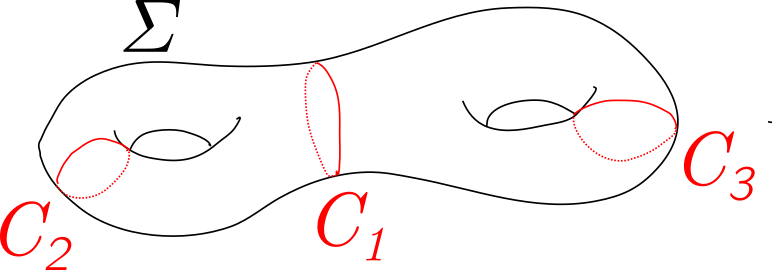
\includegraphics[width=0.5\linewidth]{genus2.png}\label{fig:genus2}}
		\subfloat[][General decomposition for $g\geq 3$.]{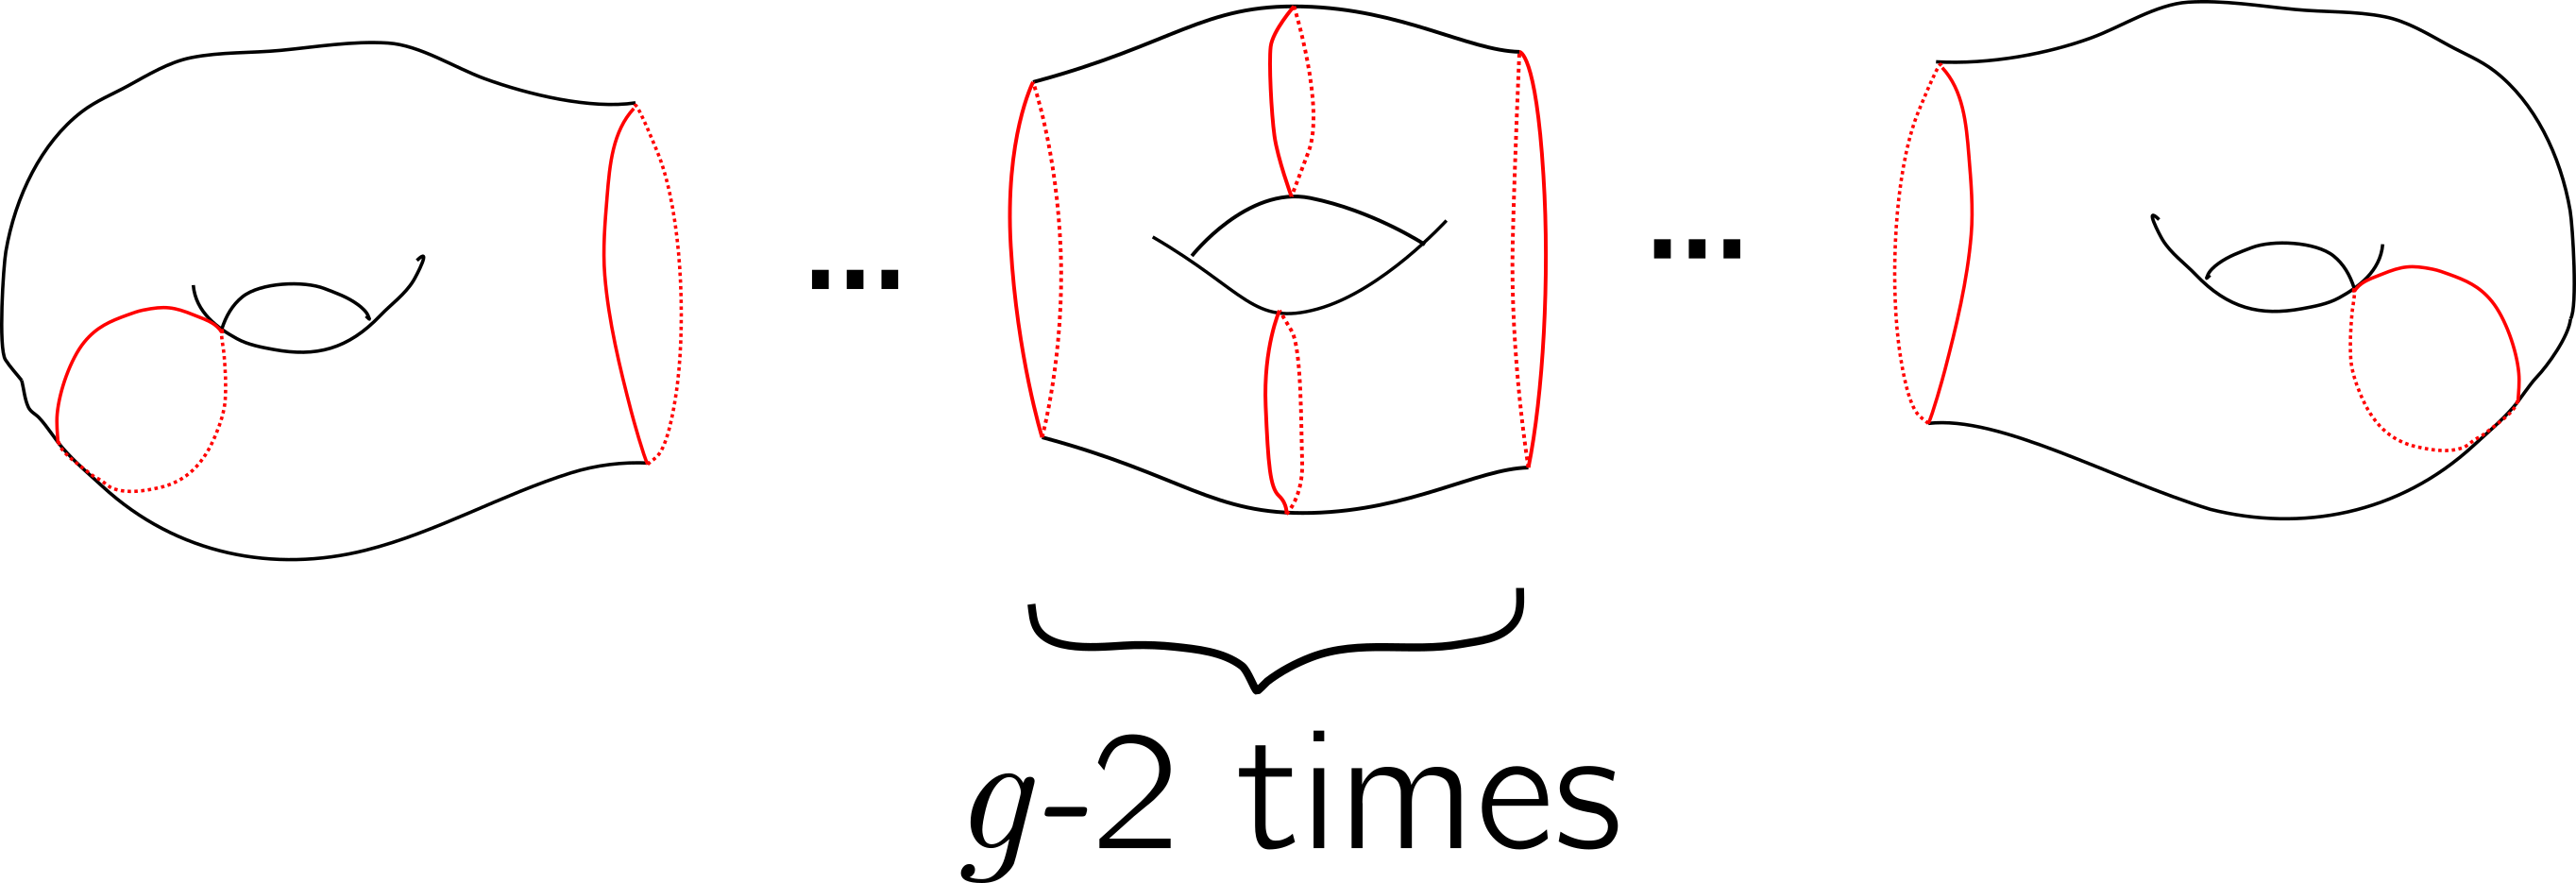
\includegraphics[width=0.5\linewidth]{genusg.png}\label{fig:genusg}}
		\caption{Decomposition of a surface $\Sigma$ into $2g-2$ trinions. }
		\label{fig:torusdecomp}
	\end{figure}

	Suppose we are given such a decomposition of $\Sigma$ into $2g-2$ trinions $D_\gamma$, $\gamma\in\{1,2,...,2g-2\}$, joined along their boundaries and with the marked points on the boundaries coinciding for any trinions with non-trivial intersection. Then the boundary circles of $D_\gamma$ give a collection $C_i$, $i\in\{1,2,...,3g-3\}$ of closed oriented curves in $\Sigma$ for which we get corresponding functions $f_i = f_{C_i}:\MM \to \mathbb{R}$ using the above definition. Since these functions are the trace of $SU(2)$ matrices, they can be described by cosine of angles $\theta_i$,
	\begin{equation}
		\theta_i(A) = \cos^{-1}(f_i(A)),
	\end{equation}
	where $\theta_i$ is taken to lie in $[0,\pi]$. This defines a map $\theta = (\theta_1,...,\theta_{3g-3}):\MM \to \mathbb{R}^{3g-3}$. These $\theta_i$ are smooth on $U_i := \theta_i^{-1}(0,\pi) \subset \MM$, which is open and dense. Thus, the Hamiltonian flows of each $\theta_i$ are defined on $\MM^{s} = \bigcap_{i=1}^{3g-3} U_i \subset \MM$. These Hamiltonian flows are periodic with constant period, which means they induce a torus action on $\MM^{s}$. Explicitly, if we let $X_i$ denote the Hamiltonian vector field of $\theta_i$, defined by
	\begin{equation}
		\iota_{X_i}\omega = d\theta_i,
	\end{equation}
	and let $e^{tX_i}$ be the corresponding vector field flow, then the action is given by $g = (\alpha_1,...,\alpha_{3g-3}) \in T^{3g-3}$ acts by
	\begin{equation}
		A \to e^{\alpha_1 X_1 + ... + \alpha_{3g-3}X_{3g-3}}A.
	\end{equation}
	 The Lie algebra of $T^{3g-3}$ is $
	\mathbb{R}^3$ and we interpret $\theta(A)$ as being dual by $\langle \theta, X \rangle = \sum \theta_i X_i$. Then
	\begin{equation}
		d\left(\langle \theta(A),X\rangle\right) = d\sum\theta_i X_i = \sum X_i d\theta_i = \iota_{X}\omega,
	\end{equation}
	which means $\theta$ is the moment map for the torus action. These functions $f_i$ also give us a real polarization of $\MM$. Let $B \subset \mathbb{R}^{3g-3}$ be the image of the $f_i$,
	\begin{equation}
		B = \{(f_i(E),...,f_{3g-3}(E))~|~ E \in \MM\},
		\label{e:B-def}
	\end{equation}
	then the fibers of the map $\pi = (f_1,...,f_{3g-3})$ foliate the smooth locus of $\MM$, and the generic fibre is a Lagrangian subvariety (cite J\&W). 
	
	Alternatively, one can describe the polarization using the picture of connections as representations of the fundamental group $\pi_1(\Sigma)$. First, a preliminary result. Let $T\subset SU(2)$ be a maximal torus.
	\begin{definition}
		A connection $A$ on $\Sigma^g$ is said to be \emph{adapted to a trinion decomposition} (a.t.d.) if there is a tubular neighbourhood $V_i \cong (-1,1)\times S^1$ of each boundary circle $C_i$ in the decomposition, such that in co-ordinates $(s,\theta)$ for $V_i$,
		\begin{equation}
			A|_{V_i} = X_i d\theta, 
		\end{equation}
		where $X_i$ is a constant element in $\mathfrak{t} = \text{Lie}(T)$.
	\end{definition}
	\begin{theorem}
		For all $y\in \pi^{-1}(b)$, there exists an adapted to trinion decomposition connection $A$ in the gauge equivalence class $y$.
	\end{theorem}
	\begin{proof}
	tbd
	\end{proof}
	
	This lets us define subgroups of $G=SU(2)$, which correspond to stabilizers of flat connections. Suppose $A$ is an a.t.d connection. Then the stabilizer of $A|_{C_i}$ in $\cG(C_i) = \Hom(C_i, G)$ consists of constant maps, and can thus be identified with a subgroup $H_i$ in $G$. If $\theta_i(A) \in \{0,\pi\}$, then $\text{hol}_{C_i}(A) = \pm\text{Id}$ and so $H_i = G$. Otherwise, $H_i = T$. 
	
	We can describe the fibre $\pi^{-1}(b)$ using these subgroups. Suppose $A$ is a.t.d. and $[A] \in \pi^{-1}(b)$. Let $\tau_i \in H_i$ for each circle $C_i$, $i\in (1,2,...,3g-3)$. Then define the map
	\begin{equation}
		\label{e:psiA}
		\psi_A : \prod_{i=1}^{3g-3} \to \pi^{-1}(b)
	\end{equation}
	as follows. Denote the trinions composing $\Sigma$ as $D_{\gamma}$, $\gamma\in{1,2,...,2g-2}$. For any circle $C_i$, let $D_{\gamma(i)}$, $D_{\gamma'(i)}$ be the trinions on either side. For $\tau=(\tau_1,\tau_2,...,\tau_{3g-3})$, choose a collection of maps $\zeta_\gamma : D_\gamma \to g$ such that for every $C_i$, $\zeta_{\gamma(i)}$ and $\zeta_{\gamma'(i)}$ are constant on a tubular neighbourhood of $C_i$, and such that
	\begin{equation}
		\zeta_{\gamma(i)}|_{C_i} = \tau_i \zeta_{\gamma'(i)}|_{C_i}.
	\end{equation}
	Here, adopt the convention that the orientation of the tubular neighbourhood is $v\wedge w$, where $w$ is tangent to the oriented circle $C_i$ and $v$ is transverse to $c_i$ and pointing \textit{into} $D_{\gamma(i)}$, thus away from $D_{\gamma'(i)}$.
	
	Now we define a connection $A_\tau$ on $\Sigma$ by defining $A_\tau$ on each trinion: $A_\tau|_{D_\gamma} := \zeta_\gamma \circlearrowright A|_{D_\gamma}$. Finally define $\psi_A(\tau) = [A_\tau]$. Next we ask, for $\tau,\tau' \in \prod_{i=1}^{3g-3} H_i$, when are $A_\tau$ and $A_{\tau'}$ gauge equivalent? 
	
	Let $J_\gamma$ be the stabilizer of $A|_{D_\gamma}$ under $\cG|_{D_\gamma} = \Hom(D_\gamma,G)$. Since $A$ is a.t.d., this also consists of constant maps. $J_\gamma = Z(G) = \{\pm \text{Id}\}$ if the holonomy is an irreducible representation of $SU(2)$, and otherwise $J_\gamma =T$ (resp $G$) if the holonomy reduces to $T$ (resp $Z(G)$).  
	
	Jeffrey and Weitsmasn give us the following lemma and theorem:
	\begin{theorem}
		If $\tau,\tau'$ are in $\prod_{i=1}^{3g-3} H_i$, then $[A_\tau] = [A_{\tau'}]$ if and only if there is a set of gauge transformations $\Phi_\gamma:D_\gamma \to G$ such that:
		\begin{enumerate}
			\item $\Phi_\gamma \in J_\gamma$ for all $\gamma$.
			\item For each boundary circle $C_i$, we have
			$$
				\Phi_{\gamma'(i)}|_{C_i} \tau_i = \tau_i' \Phi_{\gamma(i)}|_{C_i}.
			$$
		\end{enumerate}
	\end{theorem} 
	\begin{theorem}
		The map $\psi_A:\prod_i H_i \to \pi^{-1}(b)$ is surjective and the group $\prod_\gamma J_\gamma$ has a natural action on $\prod_i H_i$ so that
		\begin{equation}
			\pi^{-1}(b) = \left(\prod_i H_i\right)/\left(\prod_\gamma J_\gamma\right).
		\end{equation}
	\end{theorem}
	\begin{proof}
		jeffrey and weitsman page 600
	\end{proof}

\subsection{Moduli of Connections on a Trinion}
 	Now we've seen that the space $\MM$ can be constructed by glueing together connections defined along a trinion decomposition, so the natural question is what the space of connections on a trinion $D$, denoted $\MM(D)$, looks like. The space $\MM(D)$, like $\MM$, can be described the quotient of representations of the fundamental group into $G$ under conjugation by $G$. For a trinion, 
	\begin{equation}
		\pi_1(D) = \left\{
		[C_1], [C_2], [C_3] ~|~ [C_1][C_2][C_3]  =1
		\right\},
	\end{equation}
	where $C_i$ are the three boundary curves of the trinion. We can again define the holonomy angle functions, first letting $\tilde{\theta_i}:\Hom(\pi_1(D),G) \to [0,\pi]$ be
	\begin{equation}
		\label{e:thetacoords}
		\tilde{\theta_i}(\rho) = \cos^{-1}\left(\frac{1}{2}\Tr(\rho[C_i])\right),
	\end{equation}
	and these maps will descend under the quotient by $G$ to maps $\theta_i:\MM(D)\to [0,\pi]$. Then Jeffrey and Weitsman prove:
	\begin{theorem}
		The map $\theta = (\theta_1, \theta_2, \theta_3):\MM(D)\to[0,\pi]^3$ sends $\MM(D)$ bijectively to the set satifying the inequalities
		\begin{equation}
			|\theta_1 - \theta_2| \leq \theta_3 \leq \min(\theta_1 + \theta_2, 2\pi - (\theta_1 + \theta_2)).
			\label{e:trinion-ineqs}
		\end{equation}
		Remark that this set is a 3D simplex (insert figure?)
	\end{theorem}
	\begin{proof}
		J\&W prop 3.1
	\end{proof}
	Using this result, and the gluing process described in the last section, the image of $\MM$ under the holonomy angles $\theta_1,...,\theta_{3g-3}$ are the values satisfying the inequalities (\ref{e:trinion-ineqs}) on every trinion. Applying a theorem of Guillemin and Steinberg (cite) to this case, one obtains:
	\begin{theorem}
		\label{t:torusfibres}
		Suppose $x\in \pi(\MM) \subset B$ (defined in eqn. \ref{e:B-def}) Then
		\begin{itemize}
			\item The Hamiltonian vector fields corresponding to the functions $\theta_i$ are linearly independent on the fibre $\pi^{-1}(x)$, if and only if $x$ is a point where all the inequalities (\ref{e:trinion-ineqs}) are strict.
			\item In general, the number of linearly independent Hamiltonian vector fields on the fibre $\pi^{-1}(x)$ is equal to $3g-3-s$, where $s$ is the number of independent linear equations out of the following satisfied by $\theta(x)$:
				\begin{align*}
					\theta_{i_{\sigma(1)}(\gamma)}(x) + \theta_{i_{\sigma(2)}(\gamma)}(x)-\theta_{i{_\sigma(3)}(\gamma)}(x)&=0,\\
					\theta_{i_1(\gamma)}(x) + \theta_{i_2(\gamma)}(x) + \theta_{i_3(\gamma)}(x) = 2\pi.
				\end{align*}
			where $\sigma:{1,2,3}\to{1,2,3}$ is any cyclic permutation. These inequalities correspond to $(\ref{e:trinion-ineqs})$.
		\end{itemize}
	\end{theorem}
	Furthermore
	\begin{lemma}
		Let $x\in \MM(D)$ and let $\theta(x)$ be the holonomy angles of $x$ around the three boundary curves of $D$. Then $x$ corresponds to a conjugacy class of reducible representations of $\pi_1(D)$ if and only if at least one of the equations (\ref{e:theta-ineqs}) above is satisfied.
	\end{lemma}
	Motivated by this lemma, one defines \emph{interior triples} in $[0,\pi]^3$ to be those for which none of the equations is satisfied, i.e those on the interior of the simplex. These triples correspond to points in $\MM(D)$ which are conjugacy classes of irreducible representations of $\pi_1(D)$. Theorem \ref{t:torusfibres} tells us that the fibre $\pi^{-1}(x)$ is a torus if and only if $\theta(x)$ is an interior triple.
	\begin{theorem}
		Let $x\in B$ and let $A$ be a flat a.t.d. connection whose gauge equivalence class is in $\pi^{-1}(x)$. Further, assume that on every trinion the holonomy angles of $x$ is an interior triple. Then the fibre $\pi^{-1}(x)$ is identified with $T^{3g-3}/(\mathbb{Z}_2)^{2g-2}$ under the map $\psi_A$ defined in eqn. (\ref{e:psiA}).
	\end{theorem}
	Thus, the fibres corresponding to interior triples, which are the generic fibres, are tori of dimension $3g-3$. It is the non-generic fibres, corresponding to reducible points, which cause the result of Sniatycki to fail here.
	
	\subsection{Counting Bohr-Sommerfeld Points}
	With this real polarization of the moduli space, Jeffrey and Weitsman proceed to count the number of Bohr-Sommerfeld points \cite{jeffrey_bohr-sommerfeld_1992}. In this section we will lay out the results that we want to use going forward.
	
	\begin{definition}
		Let $(\MM,\omega)$ be a symplectic manifold with prequantum line bundle $\LL$ and polarisation $\pi:\MM\to B$. A point $b\in B$ is called a \emph{Bohr-Sommerfeld} point if $\LL|_{\pi^{-1}(b)}$ possess a one-dimensional family of global covariant constant sections.
	\end{definition}
	The quantization of a prequantum system is $\mathcal{H} = \bigoplus_{i=1}^{\dim M} H^i(M, \mathcal{J}_\pi)$, where $\mathcal{J}_\pi$ is the sheaf of sections of $\LL$ covariant constant along the fibres of $\pi$. Sniatycki's theorem \cite{sniatycki_cohomology_1977} proves that when the polarisation is a fibration, the dimension of $\mathcal{H}$ is given by the number of Bohr-Sommerfeld points. Although this result does not apply here, it still provides motivation for counting the Bohr-Sommerfeld points.
	
	For $\Sigma$ a connected compact Riemann surface of genus $g$, fix a trinion decomposition $\{D_\gamma\}$, and label the boundary loops of $D_\gamma$ as $C_{i_1(\gamma)}$, $C_{i_2(\gamma)}$ and $C_{i_3(\gamma)}$. We call a boundary loop $C_i$ \emph{separating} if removing it disconnects $\Sigma$. Recall the co-ordinates $\theta_i$ for the points $x\in \MM$ defined in equation $\ref{e:thetacoords}$. 
	\begin{theorem}[J\&W Thm 8.1]
		\label{t:bs-count}
		The set $P^{bs}$ of Bohr-Sommerfeld points in $B$ is given by the points $x\in B$ satisfying the conditions:
		\begin{enumerate}
			\item For each boundary circle $C_i$, $\theta_i(x) = \frac{\pi l_i}{k}$ for some $l_i \in \mathbb{Z}_k$, with $l_i$ even if $C_i$ is separating.
			\item For each trinion $D_\gamma$, $l_{i_1(\gamma)} + l_{i_2(\gamma)} + l_{i_3(\gamma)} \in 2\mathbb{Z}$.
		\end{enumerate}
	(what is $k$?)
	\end{theorem}
	From theorem \ref{t:torusfibres}, we know that $(\theta_1,...,\theta_{3g-3})$ is the image of a point $x\in B$ if and only if the conditions (\ref{e:trinion-ineqs}) are satisfied for the triple $(\theta_{i_1(\gamma)}, \theta_{i_2(\gamma)}, \theta_{i_3(\gamma)})$ corresponding to each trinion $D_\gamma$. We can represent a trinion decomposition as a trivalent graph, with a vertex for each trinion and an edge for each boundary circle. Therefore, a Bohr-Sommerfeld point gives a labelled trivalent graphs, where the integer $l_i$ is assigned the edge corresponding to boundary circle $C_i$. The set of Bohr-Sommerfeld points is bijective with labelled trivalent graphs whose labelling satisfy certain conditions. This picture gives the final result of Jeffrey and Weitsman:
	\begin{theorem}[J\& W Thm 8.3]
		Consider a fixed trinion decomposition of a compact connected Riemann surface $\Sigma$ of genus $g$. It gives rise to a trivalent graph, and a real polarisation of the moduli space $\MM$ of flat $SU(2)$ connections on $\Sigma$. There is one-to-one correspondence between the Bohr-Sommerfeld points of the polarisation and the set of integer labellings of the edges of the graph satisfying the conditions 1,2 in \ref{t:bs-count} and equation \ref{e:trinion-ineqs}.
	\end{theorem}
	Importantly, this theorem tells us that the Bohr-Sommerfeld points are counted inside the moment polytope defined by equation \ref{e:trinion-ineqs}. In the next section, we discuss the construction of a larger moduli space which is a smooth toric variety, allowing us to apply Sniatycki's theorem, but whose moment polytope agrees that that of $\MM$. This means the quantization of the larger moduli space has dimension given by this point-count; it will remain to show that the quantization of the larger moduli space agrees with that of $\MM$. 
	
	
%	
	
	\section{Extended Moduli Spaces of Connections}
	As always, let $\Sigma$ be a compact connected genus $g$ Riemann surface. Recall that one construction of our moduli space $\MM$ was as the representations $\Hom(\pi_1(\Sigma),G)/G$, which has its subset topology as $\xi^{-1}(e)/G \subset G^{2g}/G$, where 
	\begin{equation}
		\xi(A_1,B_1,...,A_g,B_g) = \prod_{i=1}^g A_iB_iA_i^{-1}B_i^{-1}.
	\end{equation} 
	Now let us generalize to the case where $\Sigma$ is permitted to have $n$ punctures, $\{p_i\}_{i=1}^n$. Let $c_i$ be a loop around $p_i$, and let $\{d_i\}_{i=2}^n$ be curves $d_i:p_1\to p_i$ in $\Sigma$. Then the fundamental group of $\Sigma$ can be written \cite{hurtubise_representations_2000}[2.2]:
	\begin{equation}
		\pi_1(\Sigma) = \langle a_i, b_i, c_1, d_jc_jd_j^{-1} ~|~ \prod_{i=1}^{g}a_ib_ia_i^{-1}b_i^{-1}c_1\prod_{j=2}^{n}d_jc_jd_j^{-1}=e\rangle.
	\end{equation}
	Thus, we will redefine $\xi:G^{2g+2n-1}\to G$ as
	\begin{equation}
		\xi(a_1,b_1,...,a_g,b_g,c_1,...,c_n,d_2,...,d_n) = \prod_{i=1}^{g}a_ib_ia_i^{-1}b_i^{-1}c_1\prod_{j=2}^{n}d_jc_jd_j^{-1}.
	\end{equation}
	Suppose $\{C_i\}_{i=1}^{2g-g}$ is a trinion decomposition for an unpunctured surface $\tilde{\Sigma}$. Let $\Sigma_i$ be the (singular) surface obtained by shrinking $C_i$ to a point $p_i$ (needs clarification). Then proposition \ref{t:atd-thm} tells us that any element $A$ in $\MM$ can be represented by an A.T.D. connection, meaning that $A$'s holonomy around the curve $c_i$ corresponding to the point $p_i$ is in the fundamental alcove $\Delta\subset \mathfrak{t}$. Repeating this for each $C_i$ tells us that our moduli space corresponds to the $T$-extended moduli space:
	\begin{equation}
		\MM = \MM^T := \{(A_i,B_i,D_j,C_j)\in G^{2g+n-1}\times \exp(\Delta)^n ~|~ \xi(A_i,B_i,D_j,C_j) = \mathds{1}\}.
	\end{equation}
	We can also define the $G$-extended moduli space:
	\begin{equation}
	\MM^G := \{(A_i,B_i,D_j,C_j)\in G^{2g+n-1}\times G^n ~|~ \xi(A_i,B_i,D_j,C_j) = \mathds{1}\},
	\end{equation}
	and it is clear that $\MM^T \subset \MM^G$ by including $\exp(\Delta)\subset G$. There is an action of $G^n$ on these spaces. For $(A_i,B_i,D_j,C_j)\in \MM^G$, an element $\sigma$ in the first copy of $G$ acts by:
	\begin{align*}
		A_j &\to \sigma A_j \sigma^{-1},& 	B_j&\to \sigma B_j\sigma^{-1}
	\end{align*}
	\begin{align*}
		D_j&\to \sigma D_j, & C_1 &\to \sigma C_1\sigma^{-1}
	\end{align*}
	and an element $\sigma$ in the $l$th copy $(l=2,...,n)$ of $G$ acts by
	\begin{align*}
	D_l&\to D_l\sigma^{-1}, & C_l &\to \sigma C_l\sigma^{-1}.
	\end{align*}
	This action restricts to give an action of $G^n$ on $\MM^T$. 
	
	\section{Symplectic Implosion}
	To proceed, we will state some definitions and results of (citations here):
	
	
	\begin{definition}
		For $\MM^G$ defined above, with fundamental alcove $\Delta\subset G$, we define the imploded cross section 
		\begin{equation}
			P := \prod_{\sigma} \frac{\Phi^{-1}(\sigma)}{[G_\sigma, G_\sigma]},
		\end{equation}
		where $\sigma$ ranges over the faces of $\Delta$, and $G_\sigma$ is the stabilizer of $\sigma$ under the action of $G$ by conjugation at a point in the interior of $\sigma$.
	\end{definition}
	TODO: all of this section \pagebreak
	

	
	Now associated to the compact Riemann surface $\Sigma$ we have a symplectic variety $P$ of representations with weighted frames, which is toric for $G=SU(2)$ and has a prequantum line bundle $\LL_P$ corresponding to $\LL$ on $\MM$. Now we will go in detail on the other half of Jeffrey and Hurtubise's construction, building the complex variety $\cP$ of \emph{framed parabolic bundles} over a singular curve $\tilde{\Sigma}$ corresponding to contracting the loops in a trinion decomposition of $\Sigma$. We will see that $P$ and $\cP$ are diffeomorphic, meaning that we can compute sections of prequantum line bundles over $\cP$ using the structure of $P$.
	
	First we will see how to embed $\MM$ into projective space, as this construction will have us transform the data of $\MM$ from holomorphic bundles over $\Sigma$ to sheaves, and will lay the groundwork for the embedding we will require later as a hypothesis of the theorem of Harada and Kaveh. Then we will describe the construction of $\cP$ and the diffeomorphism with $P$.
	\section{Projective Embedding of $\MM$}
	\label{s:m-embedding}
	The moduli $\MM$ of flat $SL(n,\C)$ bundles can be embedded into projective space, as we will now describe following the work of Thaddeus and Giesker (cite). First, fix a line bundle $L$ of sufficiently high degree so that for all $E\in N(k,d)$ $E\otimes L$  is globally generated (and redefine $E$). Then, for some large $N$ we can write $E$ as a quotient:
	\begin{equation}
	\phi:\OO^N \to E.
	\end{equation}
	This quotient induces a map from $\wedge^k(\OO^N) \to \wedge^k(E)$ and the $SL(k,\C)$ structure induces an isomorphism $\mu:\wedge^k(E)\cong L^k$. Hence, a quotient of the trivial bundle induces an element $\hat{\beta}$ in 
	\begin{equation}
	V_1 := \Hom(H^0(\wedge^k(\OO^N)), H^0(L^2)).
	\end{equation}
	Now to pass to $\MM$ we quotient by $GL(k,\C)$. Suppose we have $\phi_2 = \Lambda^{-1} \phi_1 \Lambda$. Then
	\begin{equation}
		\hat{\beta}_2 = \mu(\wedge^k \phi_2) = \mu(\wedge^k \Lambda^{-1}\phi_1 \Lambda) = \det\Lambda \mu(\wedge^k \phi_1) = \det\Lambda~ \hat{\beta}_1.
	\end{equation}
	Therefore the orbits of $GL(k,\C)$ correspond to equivalence classes in $\PP(V_1)$. It is this mapping, which we will denote $\iota:\MM\to \PP(V_1)$, which we claim is an embedding. 
	\begin{lemma}
		The map $\iota:\MM \to \PP(V_1)$ is injective.
	\end{lemma}
	\begin{proof}
		 Suppose $(E_1, \dbar_{E_1})$ and $(E_2, \dbar_{E_2})$ are holomorphic vector bundles for which $\hat{\beta}_1 = \iota(E_1) = \iota(E_2) = \hat{\beta_2}$. Since the $SL(k,\C)$ structure is unique up to $\C^\ast$, this means that
		\begin{equation}
		\wedge^k \phi_1 = \lambda \wedge^k \phi_2
		\end{equation}
		for some $\lambda \in \C^\ast$. Fixing a local trivialization of $E_1$, $E_1|_U \cong U\times \C^k$, and picking a local frame $e_1,..,e_k$, choose any sections $s_1,...,s_k \in \OO^N|_{U}$ so that $\phi_1(e_i) = s_i$. Let $s = s_1 \wedge s_2 \wedge ... \wedge s_k$. Then
		\begin{equation}
		e_1\wedge...\wedge s_k=\phi_1(s_1)\wedge...\wedge \phi_1(s_k)= \wedge^k \phi_1(s) = \lambda \wedge^k \phi_2(s) = \lambda \phi_2(s_1)\wedge...\wedge \phi_2(s_k)
		\end{equation}
		Since $\{e_i\}$ was a local frame, the LHS is non-zero, and thus the RHS is non-zero. Therefore $\{\phi_2(s_i)\}$ is a local frame trivializing $E_2$ on $U$. This map $e_i \to \phi_2(s_2)$ gives an isomorphism of $E_1$ with $E_2$. Note that this isomorphism is not unique as we could have picked other sections $\tilde{s}_i$ with $\phi_1(\tilde{s}_i) = e_i$.
	\end{proof}
	\begin{theorem}
		The map $\iota:\MM \to \PP(V_1)$ is an embedding.
	\end{theorem}
	\begin{proof}
		Since the lemma shows it is injective, it remains to show its derivative is everywhere injective. We give a proof following Thaddeus (GIT and flips page 717).
	\end{proof}

	\section{Parabolic Vector Bundles}
	Given a trinion decomposition of the Riemann surface $\Sigma$, let us fix the holonomies around each boundary loop. If we think of each trinion as a thrice-punctured sphere and consider the space of connections with fixed holonomies on the trinion, then due to Mehta and Seshadri (cite) there is a correspondence between the moduli of $\pi_1(\Sigma)$ representations into $SU(n)$ and that of rank-$n$ holomorphic bundles with an $SL(n,\C)$ structure and a parabolic structure at the punctures of $\Sigma$, which we call a parabolic bundle. Under this correspondence, the eigenvalues of the holonomy get translated into a set of weights for the parabolic structure. 
	
	We want to consider the moduli space of connections with all possible holonomies, and therefore we will want to fit all these moduli of parabolic bundles together, and in such a way that we can even include the $\theta_i = 0,\pi$ cases, which will correspond to weights $0$ and $1$. This is the construction of Hurtubise and Jeffrey which we will describe in the next section. First we lay out the basic definitions and results about parabolic bundles.
	\begin{definition}
		A \emph{parabolic bundle} over a complex manifold $\Sigma$ is a holomorphic vector bundle $E$ over $\Sigma$ with a \emph{parabolic structure}, which is a point of marked points $\{p_1,...,p_n\}$ and for each point, a flag of subspaces in the fibre $E_{p_k}$. 
	\end{definition}
	In particular if $E$ has rank 2, then a parabolic structure on $E$ is a choice of points $\{p_k\}$ and a sheaf homomorphism $\alpha:E\to S$ where $S := \bigoplus_{k} \C_{p_k}$.
	
	There is an adapted notion of stability for parabolic vector bundles.
	\begin{definition}
		Let $\gamma_1,...,\gamma_n \in [0,1]$ be a set of weights. For a subbundle (not neccesarily proper) $F$ of $E$ we set $\mu_i(F) = 1$ if $F_{p_i} \subset \ker\alpha_i$, and $\mu_i = 0$ otherwise. Define $\sigma(F) = \frac{1}{rk(E)}$ if $F=E$ and $0$ otherwise. Then we say a pair $(E,\alpha)$ is \emph{stable} with respect to $\gamma$ if 
		\begin{equation}
		rk(E)\deg(F) < rk(F)\left(\deg(E) - \sum_{i=1}^n \gamma_i\right) 
		+ rk(E)\sum_{i=1}^n(1 - \mu_i(F) + \sigma_i(F))\gamma_i.
		\end{equation}
		If the inequality is not strict, $(E,\alpha)$ is \emph{semi-stable}.
	\end{definition}
	This lemma of Hurtubise and Jeffrey (cite) summarizes some important results about tweighted parabolic bundles.
	\begin{lemma}
		\label{l:ss-lemma}
		If $(E,\alpha)$ is a parabolic bundle semi-stable with respect to weights $\gamma$, then:
		\begin{enumerate}
			\item The kernal of $\alpha$ is torsion free, and the torsion subsheaf of $E$ is non-zero only at the $p_i$, equalling $0$ or $\C$ at each $p_i$.
			\item If $\gamma_i >0$, then $\alpha_i \neq 0$.
			\item If $\gamma_i < 1$, then $E$ is torsion free at $p_i$.
			\item If $\gamma_i \in (0,1)$, one has a parabolic structure at $p_i$, and if all the weights are in $(0,1)$, the stability condition is identical to that of parabolic bundles with weights $(1-\gamma_i)/2$ and $(1+\gamma_i)/2$.
			\item If $(E,\alpha)$ is locally free at $p_i$ and $\alpha \neq 0$, then for $\gamma_i = 0$, there is a family $(E_t, \alpha_t)$, $t\in \C$, of semi-stable pairs such that $(E_t,\alpha_t)\cong (E,\alpha)$ for $t\neq 0$, and $\alpha_0 = 0$. 
			\item If $(E,\alpha)$ is locally free at $p_i$ and $\alpha \neq 0$, then for $\gamma_i = 1$, there is a family $(E_t,\alpha_t)$, $t\in \C$, such that $(E_t, \alpha_t)\cong (E,\alpha)$, $t\neq 0$ and $E_0$ has torsion at $p_i$.
		\end{enumerate}
	\end{lemma}
	\begin{proof}
		Hurtubise and Jeffrey (cite) lemma 4.3
	\end{proof}
	In particular, this lemma tells us that when $\gamma_i\in (0,1)$, which will correspond to connections with holonomy in $(0,\pi)$, we get well-behaved parabolic structures without torsion. It also tells us there are two edge cases to consider. When $\gamma_i = 0$, the parabolic structure vanishes, and when $\gamma_i = 1$ we acquire torsion. To fit all possible holonomies into a moduli space, each of these cases will need to be dealt with.
	
	\section{Moduli of Framed Parabolic Bundles}
	Just as we constructed the moduli space of vector bundles over a Riemann surface, let us now construct that of parabolic vector bundles. This section closely follows section 4 of Hurtubise and Jeffrey (cite). From now on, we restrict our attention to $G=SU(2)$. As always, let $\Sigma$ be a compact connected Riemann surface. Fix a line bundle $L$ of sufficiently high degree so that for all $E\in N(k,d), E\otimes L$ is a globally generated sheaf (and redefine $E = E\otimes L$). Then for some large $N$ we can write $E$ as a quotient of the trivial sheaf on $\Sigma$:
	\begin{equation}
		\phi: \OO^N \to E.
	\end{equation}
	Just as in section \ref{s:m-embedding} we have a mapping $\hat{\beta}$ taking $E$ to $V_1$. Now we add the parabolic data. At a point $p_i$, the map $\alpha_i:E\to \C_{p_i}$ pulls back to $\hat{\alpha}_i = \alpha_i\circ \phi$ in 
	\begin{equation}
		V_2 = H^0(\OO^N)^\ast.
	\end{equation}
	Since we are only interested in $\alpha_i$ up to (independent) scaling, the parabolic bundle $(E,\alpha)$ represents an equivalence class in
	\begin{equation}
		Z := \PP(V_1) \times \PP(V_2) \times ... \times \PP(V_2),
	\end{equation}
	where there are $n$ copies of $\PP(V_2)$, one for each puncture. Then letting $\tilde{\MM}$ denote the space of parabolic vector bundles, and $\tilde{\iota}:\tilde{\MM}\to Z$ denote the map taking $(E,\alpha)$ to $(\hat{\beta},\hat{\alpha})$, we get a closed subvariety $X = \tilde{\iota}\left(\tilde{\MM}\right)$ in $Z$. 

	Now we also have weights $\gamma = (\gamma_1,...,\gamma_n)$ for the parabolic structure. These vary the choice of polarization of $X$, namely the choice of line bundles on which the action of $SL(N,\C)$ \textit{linearises}. Let us recall what this means:
	\begin{definition}
		Given a linear algebraic group $G$ and a $G$-variety $X$, a line bundle $p:L\to X$ \emph{linearises} if there is an action of $G$ on $L$ such that for all $l\in L$, $g\in G$,
		\begin{equation}
			p(g\cdot l) = g\cdot p(l),
		\end{equation}
		and which restricts to a linear isomorphism $L_x \cong L_{g\cdot x}$ on fibres.
	\end{definition}
	In this case $G\cong SL(N,\C)$ which acts on $V_1$ and each copy of $V_2$.
	
	
	Let $\pi_1:Z \to \PP(V_1)$ and $\pi_{2,i}:Z\to \PP(V_2)$ denote the projections to the first factor and to the i-th factor of $Z$ respectively. Let
	\begin{equation}
		L_0 = \pi_1^\ast(\OO(N)),~ \text{ and } ~ L_{1,i} = \pi_1^\ast(\OO(N-1))\otimes \pi_{2,i}^\ast (\OO(2)).
	\end{equation}
	Then the linearisation corresponding to weights $\gamma = (\gamma_1,...,\gamma_n)$ is 
	\begin{equation}
		L_\gamma = (L_0)^{s_0} \otimes \left(
		\otimes_{i=1}^n (L_{1,i})^{s_{1,i}}
		\right),
	\end{equation}
	where $s_0(\gamma_i) = s_{1,i}(1-\gamma_i)$.
	\begin{lemma}
		$L_i$ is a linearisation of the action of $G$ on $X$.
	\end{lemma}
	\begin{proof}
		????????????/
	\end{proof}
	In summary, what we have now are a collection of moduli spaces of parabolic bundles semi-stable with respect to weights $\gamma$, with $\gamma_i \neq 0,1$. We want to fit these spaces together, and in such a way that we can include $\gamma_i = 0,1$. To do this, we put a $(\PP^1)^n$-bundle over $X$,
	\begin{equation}
		Y = \PP(L_0\oplus L_{1,1})\oplus \PP(L_0\oplus L_{1,2})\oplus ... \oplus \PP(L_0\oplus L_{1,n}).
	\end{equation}
	We endow $Y$ with the natural polarisation $\OO(1,1,...,1)$. Now $Y$ contains all the stable points for the various choice of weights, which correspond to the various possible holonomies of the unitary connections. We still need to account for gauge equivalence, which apriori suggests we take the $SL(N,\C)$ quotient. It will turn out that this is not quite correct, as we need to make an adjustment with $\gamma_i = 0,1$.
	
	Consider the space of weighted parabolic bundles as quadruples $(E, \alpha_i, A_i, \gamma)$, where $\alpha_i:E\to \C_{p_i}$ is the parabolic structure, $A_i$ is a subspace of $E_{p_i}$, with $A_i = \ker\alpha_i$ whenever $\alpha_i \neq 0$ (equiv. $\gamma \neq 0$), and $\gamma$ are the weights as usual. When $\gamma_i \neq 0$, we have not added any new information. When $\gamma_i = 0$ we are adding a projective class $A_i$ for the parabolic structure even as the map vanishes.
	
	On the other hand when $\gamma_1 = 1$, the sheaves can acquire torsion meaning they are no longer locally free. To handle this, we first need
	\begin{lemma}[H\& J Lemma 4.11]
		Let $E_t$, $t\in\C$ be a family of coherent rank 2 sheaves over $\Sigma$, with $E_t$ locally free at $p$ for $t\neq 0$, and with $E_0$ having torsion subsheaf $\C_p$ near $p$. Let $\phi_t \in H^0(\Sigma, \wedge^2(E)^\ast)$ be a family of $SL(2,\C)$ structures on $E_t$. Then $\phi_0$ vanishes at $p$.
		\label{t:sl2-lemma}
	\end{lemma}
	\begin{proof}
		If $z$ is a local co-ordinate on $\Sigma$ on an open set containing $p$, such that $z(p)=0$, one can obtain $E_t$ locally (up to reparameterization) from the exact sequence 
		\begin{equation}
			\OO \xrightarrow{(0,t^k,z)} \OO \oplus \OO \oplus \OO \xrightarrow{~~~~~}E_t
		\end{equation}
		for some integer $k$. Then the $SL(2,\C)$ structures $\phi_t$ are multiples of $e_1^\ast \wedge (-ze^\ast_2 + t^k e^\ast_3)$, which vanishes when $z=t=0$.
	\end{proof}
	Since $Y$ is a projective bundle, we can freely tensor with line bundles and write $Y$ as the bundle
	\begin{equation}
		Y = \bigoplus_{i=1}^n\PP\left(\pi_1^\ast\left(
		\OO(-1)
		\right)\oplus \pi_{2,i}^\ast\left(\OO(-2)\right)\right).
	\end{equation}
	In this form, when $\gamma \neq 1$ we have a natural lift of a parabolic bundle $(E,\alpha)\in X$ to $Y$, given by 
	\begin{equation}
		\hat{E} = \left(
		(\hat{\beta}, \hat{\alpha}_1^2),(\hat{\beta},\hat{\alpha}_2^2),...,(\hat{\beta},\hat{\alpha}^2)
		\right),
	\end{equation}
	which we want to extend to the torsion case where $\gamma = 1$. When we have torsion at say $p_i$ ($\gamma_i = 1)$, we could rescale the torsion subsheaf of $E$, modifying $\hat{\alpha}_i^2$ to $c\hat{\alpha}_i^2$ for some $c$. This rescaling should remain in the same equivalence class, and if $\hat{\beta} \neq 0$ then since $\hat{\beta}$ is not rescaled this would not be the case. Therefore we want that the $i$-th component of the lift of $E$ in $Y$ should be $(0,\hat{\alpha}_i^2)$. This is achieved as follows; recall that $\hat{\beta}$ is defined by composing
	\begin{equation}
		\wedge^2(\OO^N) \xrightarrow{\phi} H^0(\Sigma, \wedge^2 E) \xrightarrow{\xi} H^0(\Sigma, L^2)
	\end{equation}
	where $\phi:\OO^N \to E$ is a quotient defining $E$, and $\xi$ was its $SL(2,\C)$ structure. We have a commutative diagram:
	\begin{equation}
		TBD
	\end{equation}
	Then for $\gamma \neq 1$ one has $\xi = \text{ev}_\OO^{-1}\circ \xi^{p_i} \circ \text{ev}_{\wedge^2(E)}$, and so for $\gamma_i=1$ we use this definition to define $\xi^{p_i}$ at the torsion points of $E$. Then, from lemma \ref{t:sl2-lemma}, one has that $\hat{\beta}_i$ vanishes when there is torsion at $p_i$. Using this definition we can define a lift for all $(E,\alpha)\in X$ to $Y$ by $
	\hat{E} = \left(
	(\hat{\beta}, \hat{\alpha}_1^2),(\hat{\beta},\hat{\alpha}_2^2),...,(\hat{\beta},\hat{\alpha}^2)
	\right).$
	
	Next Hurtubise and Jeffrey analyse which elements of $Y$ are stable or semistable as weighted parabolic bundles. In lemma (ref) we saw that torsion in the kernal of $\alpha_i$ destabilised $(E,\alpha) \in X$. The same is true in $Y$:
	\begin{lemma}[H\&J Lemma 4.13]
		A semi-stable element $y\in Y$ corresponds to a bundle parabolic bundle $(E,\alpha)$ with no torsion in the kernal of $\alpha$.
	\end{lemma}
	To allow the the $\alpha_i$ to go to zero but still preserve the information of which projective class we have at $p_i$, we define a new map. Let $(E,\alpha)\in X$ with $SL(2,\C)$ structure $\phi$. Then we can map $(E,\alpha,\phi)\to Y$ by
	\begin{equation}
		(E,\alpha,\phi) \to \bigoplus_{i=1}^n\left(
		(\phi(p_i)^N, \phi(p_i)^{N-1}\alpha_i^2
		\right),
	\end{equation}
	and we define $\hat{Y}$ to be the closure in $Y$ of the image of this map. In this closure, we can take $\alpha_i =0$, but since $\phi(p_i)\neq 0$ we preserve the information of a subspace of $E$ at $p_i$ (unsure?). Then since $\phi(p_i)\neq 0$, lemma \ref{t:sl2-lemma} guarantees $E$ is torsion free at $p_i$. Finally the proposition regarding stability is
	\begin{theorem}[H\&J Prop 4.14]
		Let 
		\begin{equation}
			y = \left(
			(b_1, a_1), (b_2, a_2),...,(b_n, a_n)
			\right)
		\end{equation}
		be a point in $\hat{Y}$. Let $\Gamma(y)$ be the set of $\gamma_i \in [0,1]$ such that $\gamma_i =0$ if $a_i =0$ and $\gamma_i = 0$ if $b_i = 0$. Then $y$ is semi-stable if and only if for one element $\gamma \in \Gamma(y)$, $\pi(y)\in X$ is $\gamma$-semi-stable.
	\end{theorem}
	Therefore semi-stable elements in $\hat{Y}$ all project down to semi-stable elements of $X$ for some choice of weights, and the GIT quotient $\hat{Y}\sslash SL(N,\C)$ corresponds to equivalence classes of quadruples $(E,\alpha_i, \hat{\alpha}_i, \phi)$ where $(E,\alpha)$ is a parabolic bundle, $\hat{\alpha}_i$ is a subspace of $E|_{p_i}$ (which is the kernal of $\alpha_i$ when $\alpha_i \neq 0$) and $\phi$ is an $SL(2,\C)$ structure. However this is not quite the final moduli space we want to construct, as we have added the extra information of $\hat{\alpha}_i$ when $\alpha_i = 0$. At these points, $\hat{\alpha}_i \in \PP_1=\PP(E|_{p_i})$. We want to collapse these extra $\PP_1$s. To do this, embed $V_1$ into $W_1 = V_1^{\otimes N}$ so that a non-zero element $l$ in $L_{0} = \pi_1^\ast(\OO(N))$ can be thought of as an element in $W_1^\ast$ by taking $v_1\otimes...\otimes v_n$ to $l(v_1)l(v_2)...l(v_n)$. Similarly, embedding $V_2$ into $W_2 = V_1^{\otimes N-1}\otimes V_2\otimes V_2$ allows us to think of non-zero elements in $L_{1,i}$ as elements of $W_2^\ast$. Then this maps $\hat{Y}$ to a subvariety $\tilde{Y}$ in $\bigotimes_{i=1}^n \PP(W_1\otimes W_2)$, and the map collapses the unwanted $\PP_1$s while being an embedding otherwise. 
	
	Finally, we let $\cP = \tilde{Y}\sslash SL(N,\C)$ be the geometric quotient, and we call it the \emph{moduli space of framed parabolic bundles}.
	
	\section{Framed Parabolic Bundles on a Trinion}
	To understand the moduli space of framed parabolic bundles on our entire Riemann surface, it is insightful to mirror the construction of section 3 and decompose the Riemann surface into trinions. Towards this end, let us compute $\cP$ for one trinion $D$, a copy of $\PP^1$ with three marked points. Without loss of generality, let the three marked points be $z=0,1,\infty$. 
	
	\begin{lemma}
		A degree-0 framed parabolic sheaf $(E,\alpha)$ on $D$ which is semi-stable must fall into one of four cases:
		\begin{enumerate}
			\item $E$ is trivial; $E\cong \OO\oplus \OO$.
			\item $E$ is torsion-free but not trivial, and $E\cong \OO(1)\oplus\OO(-1)$.
			\item $E$ has torsion at one point $p$, and $E\cong \OO\oplus\OO(-1)\oplus \C_p$.
			\item $E$ has torsion at two points $p_1,p_2$, and $E\cong \OO(-1)\oplus\OO(-1)\oplus\C_{p_1}\oplus \C_{p_2}$.
		\end{enumerate}
	\end{lemma}
	\begin{proof}
		Suppose that $E$ has no torsion. Then $E \cong \OO(j)\oplus \OO(-j)$, $j\in\mathbb{Z}$. If $E$ is semi-stable with respect to some weights $\gamma$, the semi-stability condition is that for all subbundles $F$ of $E$,
		\begin{equation}
			2\deg(F) \leq rk(F)\left(
			0-\sum_{i=1}^n \gamma_i
			\right) + 2\sum_{i=1}^n(1-\mu_i(F) + \sigma(F))\gamma_i,
		\end{equation}
		where we recall that $\sigma(F) = \frac{1}{rk(E)}$ if $F=E$ and $0$ otherwise, and $\mu_i(F) = 1$ is $F_{p_i} \subset \ker \alpha_i$ and $0$ otherwise. Consider $F = \OO(j)$. The equation becomes
		\begin{equation}
			2j \leq \sum_{i=1}^n \gamma_i - 2\mu_i(F).
		\end{equation}
		Since $\gamma_i \leq 1$, This can never be satisfied for $j \geq 2$, and therefore $E = \OO\oplus\OO$ or $E=\OO(1)\oplus\OO(-1)$ are the only choices which can yield a semi-stable parabolic sheaf. 
		
		When $E$ has torsion at one of the marked points, say $p$, then let $E' = E/\text{Tor}(E)$.
		which is a bundle with $E\cong \OO(j-1)\oplus\OO(-j)$. Let $F=\OO(j-1)\oplus \C_p$. Then the stability condition for $E$ and $F$ is
		\begin{equation}
			2j \leq \sum_{i=1}^3 \gamma_i -2\mu_i(F)
		\end{equation}
		The right-hand side is at most 3, and therefore if $j\geq 2$ then the sheaf $\OO(j-1)\oplus \C_p$ is destabilising. Therefore we must have $E' \cong \OO(-1)\oplus \OO$, and $E \cong \OO(-1)\oplus \OO \oplus \C_p$. 
		
		If $E$ has two torsion points, then $E'\cong \OO(-j)\oplus\OO(j-2)$ If $j\geq 2$, then $\OO(j-2)\oplus \C_{p_1}\oplus \C_{p_2}$ will be destabilizing. If $j=0$, then $F=\OO\oplus\C_{p_1}\oplus \C_{p_2}$ has stability condition
		\begin{equation}
			4 \leq \sum_{i=1}^3 \gamma_i - 2\mu_i(F).
		\end{equation}
		The left hand side is at most 3, so $F$ is destabilizing. So $E' \cong \OO(-1)\oplus \OO(-1)$ is the only semistable choice, and $E \cong \OO(-1)\oplus \OO(-1)\oplus \C_{p_1} \oplus \C_{p_2}$. 
		
		Finally, if $E$ has torsion at all three marked points, $E' = \OO(-j)\oplus \OO(j-3)$. Then from lemma \ref{l:ss-lemma}, $\gamma_i = 1$ for all $i$, $\mu_i = 0$ for all $i$.  Therefore the stability condition for the subsheaf $F=\OO(j-3)\oplus\C_{0}\oplus \C_{1}\oplus \C_{\infty}$ becomes
		\begin{equation}
			2j \leq -3 + 2(3) = 3
		\end{equation}
		This rules out $j\geq 2$. For $j=0,1$ the subsheaf $\OO(-j)\oplus\text{Tor}(E)$ will be destabilizing; the stability condition is
		\begin{equation}
			2(3-j) \leq 3.
		\end{equation}
		Hence there are no semi-stable sheaves $E$ with torsion at three points.
	\end{proof}
	The lemma gives us the following corollary.
	\begin{theorem}
		For all degree-0 semi-stable parabolic sheaves $(E,\alpha)$ over $D$, $E\otimes \OO(1)$ is generated by four global sections. In particular, there is an exact sequence:
		\begin{equation}
		\OO(-2)\oplus \OO(-2) \xrightarrow{Az+Bz^{-1}} \OO(-1)^{\oplus 4} \xrightarrow{} E \to 0.
		\end{equation}
		With $A,B$ represented by 4x2 matrices. The map $\OO(-2)\oplus \OO(-2) \xrightarrow{Az+Bz^{-1}} \OO(-1)^{\oplus 4}$ is injective as a map of bundles away from the torsion points of $E$.
	\end{theorem}
	\begin{proof}
		From the lemma, $E\otimes \OO(1)$ falls into one of four cases, each of which is a subsheaf of $\OO^{\oplus 4}$. Each case gives us an exact sequence:
		\begin{enumerate}
			\item $\OO\oplus \OO\to \OO^{\oplus 4}\xrightarrow{} E\otimes\OO(1) \to 0$
			\item $\OO\oplus\OO(-1) \to \OO^{\oplus 4}\xrightarrow{} E\otimes\OO(1)  \to 0$
			\item $\OO\oplus\OO(-1) \to \OO^{\oplus 4}\xrightarrow{} E\otimes\OO(1) \to 0$
			\item $\OO(-1)\oplus (-1)\to \OO^{\oplus 4}\xrightarrow{} E\otimes\OO(1) \to 0$
		\end{enumerate}
		However since $\OO \hookrightarrow \OO(-1)$, we always have the fourth sequence. Tensoring it with $\OO(-1)$ we obtain the sequence in the theorem.
		
		Since $E$ is rank 2 away from torsion, and $E = \OO(-1)^{\oplus 4}/\text{im}(Az+Bz^{-1})$ by exactness, at every point $p$ without torsion $\text{im}(Az+Bz^{-1})|_p = \text{im}(Ap+Bp^{-1})$ has dimension 2. The domain $\OO(-2)\oplus\OO(-2)|_p$ has dimension 2, and so by rank-nullity theorem the kernal of $Ap+Bp^{-1}$ has dimension $2-2=0$ and is hence injective. 
	\end{proof}
	The 4x2 matrices $A,B$ depend on $E$ and in fact determine $E$. The parabolic structure $\alpha = (\alpha_0,\alpha_1,\alpha_\infty)$ is realized as maps $\OO(-1)^{\oplus 4}\to \C_{p_i}$ for which $\text{im}\left(\OO(-2)\oplus\OO(-2)\right) \subset \ker\alpha_{p_i}$. These maps are represented by row vectors $V_0,V_1,V_\infty$ in $\C^4$ satisfying the conditions:
	\begin{align}
		V_0 A &=0, & V_1(A+B) &= 0, & V_\infty B &=0.
	\end{align}
	
	Finally, the framing ($SL(2,\C)$ structure) is determined by the isomorphism
	\begin{equation}
		\wedge^2 (E) \cong \left(\wedge^2 \OO(-2)\oplus \OO(-2)\right)^\ast\otimes \wedge^4\OO(-1)^{\oplus 4},
	\end{equation}
	so the data of $A,B, V_0,V_1$ and $V_\infty$ determines a framed parabolic bundle.
	
	There is an action of $GL(2,\C)\times GL(4,\C)$ on this data, by
	\begin{equation}
		\label{e:p3-conds}
		(g,G)\cdot (A,B,V_0,V_1,V_\infty) = (GAg^{-1}, GBg^{-1}, V_0G^{-1}, V_1G^{-1}, V_\infty G^{-1}),
	\end{equation}
	and the orbits of this action are the isomorphism classes of framed parabolic bundles we are interested in. We define four functions which are projectively invariant under this action:
	\begin{align}
		\label{e:p3-coords}
		x&=\det(A,B),& y&=\det\begin{pmatrix}
		V_0 A\\
		V_1 B\\
		\end{pmatrix}, & z&= \det\begin{pmatrix}
		V_0 B\\
		V_\infty A\\
		\end{pmatrix}, & w&= \det\begin{pmatrix}
		V_1 A\\
		V_\infty B\\
		\end{pmatrix}.
	\end{align}
	The action of $(g,G)$ on these functions pulls out the determinants of $g$ and $G$, so we can instead consider just the orbits of equivalence classes of $(x,y,z,w) \mod \C^\ast$ under the action of $SL(2,\C)\times SL(4,\C)$. 
	\begin{theorem}
		\label{t:p3-iso}
		The map $\Phi:\cP|_D$ taking a framed parabolic sheaf $(E,\alpha)$ to the class $[x:y:z:w]$ as defined in equations \ref{e:p3-coords} is an isomorphism of $\cP|_D$ with $\PP^3$. 
	\end{theorem}
	\begin{lemma}
		A point in $\cP|_D$ defined by $(A,B,V_0,V_1,V_\infty)$ is semi-stable if and only if one of the co-ordinates $x,y,z$ or $w$ is non-zero. This tells us $\Phi$ is well defined.
	\end{lemma}
	\begin{proof}
		In this proof we will use another characterization of stability, which is that $E$ is semi-stable if the closure of $\text{Orb}_G(E)$ does not contain zero, and $E$ is stable if the stabilizer is finite. 
		
		If $(A,B,V_0,V_1,V_\infty)$ defines an unstable bundle, we want to show that all the co-ordinates vanish. Suppose the closure of $(A,B,V_0,V_1,V_\infty)'s$ orbit under $SL(2,\C)\times SL(4,\C)$ contains $(0,0,0,0,0)$. First suppose the orbit itself contains $0$. Then there is $G\in SL(4,\C)$ such that $V_i G^{-1} =0$, and since $G$ is invertible this means $V_i = 0$ for all $V_0,V_1,V\infty$; this makes $y,z,w$ all 0. Furthermore, if $g\in SL(2,\C)$ such that $GAg^{-1} = GBg^{-1} =0$ then $A=B=0$ by invertibility of $G$ and $g$. Hence $x=0$; so if the orbit contains $0$ then $x=y=z=w=0$. 
		
		Now suppose that $0$ is in the closure of the orbit. This means there is a sequence of matrices $(G_i,g_i)_{i=1}^\infty$ which approach matrices which send $(A,B,V_0,V_1,V_\infty)$ to $0$. By the previous argument, either $G$ or $g$ is not invertible, or all the co-ordinates $x,y,z,w$ equal 0. Since the determinant is a continuous function on $SL(n,\C)$, the limit of the determinant is the determinant of the limit, and since $G_i$ and $g_i$ all have determinant $1$, so does their limit. They must be invertible, and hence $x=y=z=w=0$.\vspace{1em}
		
		
		Conversely, consider a point whose co-ordinates all vanish. This tells us that there is a basis of $\C^2$ for which $V_i A = (a_i,0)$ and $V_i B = (b_i ,0)$ for $i=0,1,\infty$. Pick a basis for $\C^4$ in which each $V_i$ has the form $(\ast,\ast,\ast,0)$. Then let $n>0$ and $G(z) = \text{diag}(z^{-n}, z^{-n}, z^{-n}, z^{3n})$. $G(z)$ is a one parameter family in $SL(4,\C)$ for which $G^{-1}(z)V_i \to 0$ as $z\to 0$. Let $g(z) = \text{diag}(z^{-m}, z^{m})$ for some $n < m < 3m$. Then
		\begin{equation}
			GAg^{-1}(z) =
			\begin{pmatrix}
			z^{m-n} A_{11} & z^{-m-n}A_{12}\\
			z^{m-n} A_{21} & z^{-m-n}A_{22}\\
			z^{m-n} A_{31} & z^{-m-n}A_{32}\\
			z^{m+3n} A_{41} & z^{3n-m}A_{42}\\
			\end{pmatrix} 
		\end{equation}
		If the span of the $V_i$ is 3-dimensional, then in our basis we must have $A_{12}=A_{22}=A_{32}=0$ from equation \ref{e:p3-conds}. In this case, as $z\to 0$ we have $GAg^{-1}(z) \to 0$, so this family $(G,g)(z)$ is destabilizing. If the span is 2-dimensional, $A_{32}$ may be non-zero. In this case, we modify $G(z) = \text{diag}(z^{-n}, z^{-n}, z^n, z^n)$ and get a destablizing family. Similarly, if the span of the $V_i$ is 1-dimensional, then $A_{12}=0$ and we let $G(z) = \text{diag}(z^{-3n}, z^n, z^n, z^n)$ to get a destabilizing family. All this holds for $B$ as well.
		
		In the last case with all $V_i=0$, we need only consider $A$ and $B$. Since $\det(A,B) = 0$, there is a basis in which
		\begin{equation}
			(A,B) = 
			\begin{pmatrix}
		A_{11} & A_{12}	& B_{11} & B_{12}\\
		A_{21} & A_{22} & B_{21} & B_{22}\\
		A_{31} & A_{32} & B_{31} & B_{32}\\
		A_{41} & A_{42} & B_{41} & B_{42}\\
			\end{pmatrix}
		\end{equation}
		has a row of zeros. Suppose without loss of generality it is the last row. Then let $0 < m < n$ and let $G(z) = \text{diag}(z^{n}, z^{n}, z^{n}, z^{-3n})$ and $g(z) = \text{diag}(z^{-m}, z^{m})$. The family $(G,g)(z)$ will destabilize $(A,B,0,0,0)$. 
	
	\end{proof}
	Now we prove theorem \ref{t:p3-iso}.
	\begin{proof}
		If we fix one of $x,y,z$ or $w$ to equal 1, then we are left with an open affine in $\PP^3$ isomorphic to $\C^3$. From the lemma we know $\Phi$ patches together correctly on the intersections of these affines, so if we can prove it is bijective on each affine then it will be bijective everywhere. 
	\end{proof}
	Our moduli space is therefore $\cP|_D \cong \PP^3$ over the trinion $D$. We also have an action of $(\C^\ast)^3$ on $\cP|_D$ where each factor scales the parabolic structure at one point; for $\lambda_i\in \C^\ast$,
	\begin{equation}
		(\lambda_1,\lambda_2,\lambda_3)\cdot (A,B,V_0,V_1,V_\infty) = (A,B,\lambda_1 V_0, \lambda_2 V_1, \lambda_3 V_\infty).
	\end{equation}
	In terms of our co-ordinates for $\PP^3$, the action is given by
	\begin{equation}
		(\lambda_1, \lambda_2,\lambda_3)\cdot [x:y:z:w] = [x:\lambda_1\lambda_2 y: \lambda_1\lambda_3 z: \lambda_2\lambda_3 w].
	\end{equation}
	Consider the line bundle $\OO(1)$ of homogeneous linear functions over $\PP^3$. The action on $\PP^3$ linearizes on $\OO(1)$; if $ax+by+cz+dw \in \OO(1)(\PP^3)$ then define
	\begin{equation}
	(\lambda_1, \lambda_2,\lambda_3) \cdot (ax+by+cz+dw) = ax +b\lambda_1\lambda_2 y + c\lambda_1\lambda_3 z + d\lambda_2\lambda_3 w. 
	\end{equation}
	
	\section{Gluing $\cP$ over Trinions }
	Given two Riemann surfaces $\Sigma_1$, $\Sigma_2$ with marked points $p_1$ and $p_2$, we can glue them together by identifying $p_1$ and $p_2$ to form $\Sigma = \Sigma_1 \coprod \Sigma_2 / (p_1 \sim p_2)$. This will be a nodal complex curve. If $\cP_1$ and $\cP_2$ denote the moduli space of parabolic sheaves corresponding to $\Sigma_1$ and $\Sigma_2$, we can also consider gluing them together. For framed parabolic sheaves $(E_i,\alpha_i)$, with $E_i$ over $\Sigma_i$ and $\alpha_i:(E_i)|_{p_i}\to \C$, we can combine the two into a diagram:
	\begin{equation}
		(E_1)|_{p_1} \to \C \rightarrow (E_2)|_{p_2}.
	\end{equation}
	We consider two such diagrams to be equivalent if the framed parabolic bundles on each surface are isomorphic, and if the induced maps $(E_1)|_{p_1}/\ker(\alpha_1) \to (E_1)_{p_1}/\ker(\alpha_1)$ are the same. Then taking equivalence classes under this equivalence amounts to quotienting out the anti-diagonal action of $\C^\ast$ on the framing at $p_0$ and $p_1$, and we have $\cP_{\Sigma} = \cP_0 \times \cP_1 \sslash \C^\ast$. 
	
	In particular, given a compact Riemann surface $\Sigma$ with trinion decomposition $\{D_\gamma\}_{\gamma=1}^{2g-2}$, we can pinch the boundary circles ${C_i}_{i=1}^{3g-3}$ down to points to obtain a singular surface $\tilde{\Sigma}$, consisting of $2g-2$ copies of $\PP^1$ with three marked points glued along those $3g-3$ total marked points. Then we can obtain the moduli space $\cP$ for $\tilde{\Sigma}$ by gluing the moduli spaces $\cP_\gamma$ for each trinion $D_\gamma$. From the previous section we know each $\cP_\gamma$ is isomorphic to $\PP^3$. Heuristically, this lets us estimate the dimension of $\cP$ as follows. We have a total of $3(2g-2)$ dimensions for the $\PP^3$ over each trinion, and we have to quotient an action of $\C^\ast$ along $3g-3$ curves. Therefore, we expect that $\cP$ has dimension $3(2g-2)-3g-3 = 3g-3$, which agrees with our dimension calculation for the moduli space $\MM$ from section 2 and 3. \vspace{1em}
	
	Given two trinions $D_1$, $D_2$ with moduli spaces $\cP_1 \cong \cP_2 \cong \PP^3$, each of which has their own twisting sheaf $\OO(1)$, we can ask if we get a twisting sheaf exhibiting $\cP_1 \times \cP_2 \sslash \C^\ast$ as a quasi-projective scheme. The Segre embedding lets us embed $\PP^3 \times \PP^3$ into $\PP^{15}$, which has its own twisting sheaf $\OO(1)_{\PP^{15}}$. To recall, if $[x:y:z:w]$ and $[x':y':z':w']$ are co-ordinates for each copy of $\PP^3$, then the Segre embedding is the map
	\begin{equation}
		([x:y:z:w], [x':y':z':w']) \to [xx':xy':xz':xw':yx':...:ww'],
	\end{equation}
	where the right-hand side is ordered lexicographically. Let $X$ denote the image of $\PP^3\times \PP^3$ in $\PP^{15}$ and let $p:X\to \PP^3$ denote the projection onto one factor. The Segre embedding has the property that (cite)
	\begin{equation}
		\OO(1)_{\PP^{15}}|_X = p^\ast \OO(1) \otimes p^\ast \OO(1).
	\end{equation}
	To do just one case, suppose the gluing of $D_1$ and $D_2$ is at the point $0$ in both trinions, so that the antidiagonal $\C^\ast$ action is
	\begin{align*}
		\lambda \cdot [x:y:z:w] &\to [x:\lambda y:\lambda z: w]\\
		\lambda \cdot [x':y':z':w']&\to [x:\frac{1}{\lambda}y': \frac{1}{\lambda}z':w'],
	\end{align*}
	then this gives a corresponding action on $\OO(1)_{\PP^{15}}$, whose sections are linear combinations of the co-ordinate functions on $X$. The GIT quotient is then defined as
	\begin{equation}
		X\sslash \C^\ast := \text{Proj}\left(\bigg(\bigoplus_{n\geq 0} \Gamma(X, \left(\OO(1)_{\PP^{15}}|_X\right)^n)\bigg)^{\C^\ast}\right).
	\end{equation}
	The twisting sheaf of $X\sslash \C^\ast$ is exactly the degree-0 component of this ring, with sections $\Gamma(X, \left(\OO(1)_{\PP^{15}}|_X\right)^{\C^\ast}.$ Looking at the antidiagonal action when both points are $0$, we see the invariant sections of $\OO(1)_{\PP^{15}}|_X$ are those with no $y,z,y'$ or $z'$ components, i.e:
	\begin{equation}
		\Gamma(X, \left(\OO(1)_{\PP^{15}}|_X\right))^{\C^\ast} = \text{span}(xx',xw',wx',ww').
	\end{equation}
	
	In the full-trinion decomposition setting, repeating this process at each point gives us the moduli space $\cP$ with a very ample line bundle $\LL$ embedding $\cP$ into a large projective space. Any Fubini-Study metric on that projective space gives $\LL$ a Chern connection $\theta \in \Omega^{1,1}(T^\ast \cP)$ such that $i\theta$ is a metric for $\cP$. The complex structure and metric also yield a symplectic form $\omega$ for $\cP$. Later, we will want to check that when a point in $\cP$ is a stable point in $\MM$, this symplectic form agrees with the Atiyah-Bott form on $\MM$.

%\printbibliography
\end{document}
